%%%%%%%%%%%%%%%%%%%%%%% file template.tex %%%%%%%%%%%%%%%%%%%%%%%%%
%
% This is a general template file for the LaTeX package SVJour3
% for Springer journals.          Springer Heidelberg 2010/09/16
%
% Copy it to a new file with a new name and use it as the basis
% for your article. Delete % signs as needed.
%
% This template includes a few options for different layouts and
% content for various journals. Please consult a previous issue of
% your journal as needed.
%
%%%%%%%%%%%%%%%%%%%%%%%%%%%%%%%%%%%%%%%%%%%%%%%%%%%%%%%%%%%%%%%%%%%
%
\RequirePackage{fix-cm}
%
%\setlength\textwidth{140mm}
%\documentclass[]{svjour3}                     % onecolumn (standard format)
%\documentclass[smallcondensed]{svjour3}     % onecolumn (ditto)
%\documentclass[smallextended]{svjour3}       % onecolumn (second format)
\documentclass[twocolumn]{svjour3}          % twocolumn
%\setlength\textwidth{140mm}
%\setlength\textwidth{158.7mm}
%%%%%%%%%%%%%%%%%%%%%%%%%%%%%%%%%%%%%%
%%%%%%%%%%%%%%%%%%%%%%%%%%%%%%%%%%%%%%
%FINAL VERSION:
%look for numbered but unlabelled equations
%\usepackage{refcheck}%compile twice in order to see the effects
%Acknowledgments

\usepackage{epstopdf}% To incorporate .eps illustrations using PDFLaTeX, etc.
%\usepackage{subfigure}% Support for small, `sub' figures and tables

%
\smartqed  % flush right qed marks, e.g. at end of proof
%
\usepackage{graphicx}
%
% \usepackage{mathptmx}      % use Times fonts if available on your TeX system
%
% insert here the call for the packages your document requires
%\usepackage{latexsym}
% etc.
%
% please place your own definitions here and don't use \def but
% \newcommand{}{}
%

\usepackage[labelfont=bf]{caption}
%\usepackage{capt-of}
\usepackage{subcaption} %for subfigure
\usepackage{hyperref}
\hypersetup{
    colorlinks=true,
    linkcolor=blue,
    filecolor=blue,      
    urlcolor=blue,
    citecolor=blue
}

\usepackage{natbib}% Citation support using natbib.sty
\bibpunct[, ]{(}{)}{,}{a}{}{,}% Citation support using natbib.sty
\renewcommand\bibfont{\fontsize{10}{12}\selectfont}% Bibliography support using natbib.sty


\usepackage{xurl} %make a link to break at the page margin
\usepackage{booktabs} %for \toprule

\usepackage{enumitem} % for environment enumerate, \begin{itemize}
\setlist[enumerate]{itemsep=0mm}



%\theoremstyle{plain}% Theorem-like structures
%\newtheorem{theorem}{Theorem}[section]
%\newtheorem{lemma}[theorem]{Lemma}
%\newtheorem{corollary}[theorem]{Corollary}
%\newtheorem{proposition}[theorem]{Proposition}
%
%\theoremstyle{definition}
%\newtheorem{definition}[theorem]{Definition}
%\newtheorem{example}[theorem]{Example}
%
%\theoremstyle{remark}
%\newtheorem{remark}{Remark}
%\newtheorem{notation}{Notation}


\usepackage{xspace}
\usepackage{mathtools}
\usepackage{fancyvrb} 
% for \begin{Verbatim} environment; color in verbatime
%\usepackage[T1]{fontenc}
\usepackage[defaultlines=3,all]{nowidow}

\usepackage{xcolor,listings}
\usepackage{textcomp}
\lstset{upquote=true}

\usepackage{url}

%so that we have more tolerance for large figures
%large figure is less likely to push to the end of the document
\renewcommand{\textfraction}{0.01}
\renewcommand{\topfraction}{0.99}
\renewcommand{\bottomfraction}{0.99}
\renewcommand{\dbltopfraction}{0.99} % fit big float above 2-col. text

\graphicspath{{images/}}

\newcommand{\Astar}{A$^{\!\star}$\xspace}

\newcommand{\e}[1]{\times 10^{#1}}
\newcommand{\fig}{Figure~}
\newcommand{\eq}{Equation~}
\newcommand{\fo}{Formula~}
\newcommand{\sect}{Section~}
\newcommand{\tabl}{Table~}
\newcommand{\tabls}{Tables~}
\newcommand{\chap}{Chapter~}
\newcommand{\figs}{Figures~}
\newcommand{\eqs}{Equations~}
\newcommand{\fos}{Formulas~}
\newcommand{\sects}{Sections~}
\newcommand{\appx}{Appendix~}

\newcommand{\chaps}{Chapters~}
\newcommand{\p}{p.~}
\newcommand{\pp}{pp.~}
\newcommand{\eg}{e.g.,}
\newcommand{\ie}{i.e.,}


\newcommand*{\mine}[1]{{\color{red}#1}}
%\newcommand*{\mine}[1]{{#1}}

\makeatletter
\def\verbatim@font{\normalfont\rmfamily}
\makeatother


% Insert the name of "your journal" with
 \journalname{Journal of Geovisualization and Spatial Analysis}
%

%\usepackage[disable]{todonotes}
\usepackage[]{todonotes}

\begin{document}

\title{Generalizing simultaneously to support smooth zooming:
Case study of merging area objects%\thanks{Grants or other notes
%about the article that should go on the front page should be
%placed here. General acknowledgments should be placed at the end of the article.}
}
%\subtitle{Do you have a subtitle?\\ If so, write it here}

 % if too long for running head
%\titlerunning{Generalizing simultaneously to support smooth zooming}       


%\author{Dongliang Peng *\thanks{* Corresponding author}         \and
%        Martijn Meijers \and
%        Peter van Oosterom
%}s

% if too long for running head
\authorrunning{Authors}
%\authorrunning{Dongliang Peng, Martijn Meijers, Peter van Oosterom} 

\institute{
%Dongliang Peng, Martijn Meijers, Peter van Oosterom \at
%  GIS Technology, Faculty of Architecture and the Built Environment,
%  Delft University of Technology, 
%  Julianalaan 134, Delft, The Netherlands \\
%  \email{\{D.L.Peng, B.M.Meijers, P.J.M.vanOosterom\}@tudelft.nl}  \\
}

\date{Received: date / Accepted: date}
% The correct dates will be entered by the editor





\maketitle


%\section*{Compliance with Ethical Standards}
%This research work is carried out in compliance with transparency, moral
%values, honesty, and hard work. No human participation or animals are
%involved in this research work.
%
%\section*{Funding}
%This work is part of the research programme Maps4Society with project 
%number 17644, which is (partly) financed by the Dutch Research Council 
%(NWO).
%
%\section*{Acknowledgements}
%We thank Radan \v{S}uba for partly creating the data used in our case study.
%
%\section*{Conflict of Interest}
%The authors declare that they have no conflict of interest.
%
%\section*{Ethical Approval}
%As per the literature review, this is neither a repetition
%of any work nor copied key data from other's work. The methodology,
%findings, and conclusions made here belong to original research work as
%per our knowledge and belief.
%
%\section*{Informed Consent}
%Every step of processing for publication informed to
%all co-authors of this paper at the earliest, and everything is carried out
%with collective decision and consent.
%
%
%\clearpage

\begin{abstract}
When users zoom in or out on a digital map,
the map should change correspondingly to present
geographical information at proper levels.
A way to help map users better keep track of their interested objects
is to change the map smoothly instead of 
discretely switching between several levels of detail.
This paper focuses on the problem of 
providing smooth merging of area objects.
We propose to merge multiple areas simultaneously
to share their animation durations.
In this way, each merging operation can be prolonged,
and it is visually smoother.
We present a greedy algorithm to decide 
which areas should be merged at each step.
The merging process is pre-computed 
and is recorded into a space-scale cube (SSC).
When a user accesses our web map, 
the SSC is sent to the client side 
so that the map can be generated 
by slicing the SSC in the Graphics Processing Unit (GPU).
We also explain how to snap the zooming to valid states
so that the zooming will not stop half-way of the merging operations.
Our case study shows that 
it is visually smoother to merge simultaneously
than to sequentially merge each pair of areas.
%We consider that generalizing simultaneously
%is an important step towards continuous map generalization.
%For zooming out, we merge the relatively unimportant areas into 
%their neighbors to form larger areas.
%In order to provide small and smooth changes,
%this paper merges a pair of areas by expanding one
%(winner) over the other (loser).
%At the same time, the loser gradually adapts its color to the winner.
\keywords{Space-scale cube \and vario-scale map 
\and continuous map generalization
\and web map \and simultaneous generalization}
\end{abstract}

\section{Introduction}
\label{sec:introduction}

%\textbf{display triangles in the SSC examples}

%{\color{red}Quote the changes and explanations.
%    color the references.
%    middle solution:sequence of all changes vs. all changes happen together}

When users are reading a digital map,
they expect different levels of detail (LoDs) depending on the scale.
For example, they may want to see individual buildings when zooming in
and see built-up areas when zooming out.
That is why depicting geographical information is dependent on the scale
\citep{Muller1995Generalization,Weibel1997}. 
In order to prepare map data for different scales,
a detailed map is generalized to generate coarser data 
for maps at smaller scales,
which is known as map generalization.
\citet{Mackaness2017Generalization} gave a taxonomy of 
generalization algorithms, 
including selection, simplification, aggregation, and so on.
Often, a multi-representation database (MRDB) is utilized to store
map data of different scales, 
and the proper data is sent to clients on request
\citep[\eg][]{Hampe2004multiple}.
As a result, the scale transition of a map is realized by switching 
between different LoDs. 
However, that strategy often brings large and discrete changes, 
which confuse users.
In order to provide users with better experience of zooming,
we propose to realize the scale transition with smooth changes.
In other words, each object on the map should be changed smoothly
when the scale changes.
For example, a smooth way to simplify a polyline is 
to move some of the vertices to a straight line,
and a smooth way to make a polygon disappear is to fade it out.
Because all the objects are changed smoothly,
users can keep track of their interested objects more easily.
The technology to realize the smooth scale transition is known as
\emph{continuous map generalization} (CMG).
Algorithms of CMG have been proposed 
to morph raster maps
\citep[\eg][]{Pantazis2009a,Pantazis2009b}, 
to morph polylines
\citep[\eg][]{Noellenburg2008,Peng2013LSA,Deng2015,Li2017Annealing,Li2018Fourier},
to generalize buildings
\citep[\eg][]{Li2017_Building,Peng2017Building,Touya2017Progressive},
to transform road networks or river networks
\citep[\eg][]{Suba2016Road,Chimani2014Eat,Huang2017Matrix,Peng2012River},
and to morph administrative boundaries
\citep[\eg][]{Peng2016Admin}.
Recently, \citet{Shen2020Collapse} proposed a method 
to progressively collapse rivers based on superpixels.
%Using different sizes of superpixels,
%that method is able to identify the levels of the river areas.
%As a result, that method collapses the river areas at the corresponding scales.
Further, CMG can be also used 
to simulate some temporal evolution of phenomena,
for example, how a flooding submerges the land.


Area objects are important features on maps. 
When users zoom out,
some area objects become too tiny to be seen,
which results in visual clutter.
The clutter can be avoided by generalizing the 
area objects.
The generalization operators include
merging \citep[\eg][]{HaunertWolff2010AreaAgg}, 
amalgamating \citep[\eg][]{Ware1995Areal}, 
aggregating \citep[\eg][]{Peng2017Building}, 
splitting \citep[\eg][]{Meijers2016Split}, 
and collapsing \citep[\eg][]{Haunert2008Skeleton}.
However, if zooming is realized by switching between
some levels of map representations, 
large and discrete changes usually happen.
This kind of changes may cause users to lose track of
their area objects of interest \citep{vanKreveld2001}.
In order to solve this problem, 
we smoothly and simultaneously generalize the area objects.
In our setting, each of the area objects has its \emph{semantic property},
which is also called the \emph{class} (\eg\ lake, building, and grassland).


The main contribution of this paper is 
to generalize simultaneously,
which is the first time that the simultaneity is explicitly proposed.
Because of the simultaneity,
each generalization operation has more time to take place
and thus expands in more animation frames,
which makes the generalization operation visually smoother.
The reasoning is as following, taking merging as an example.
For zooming out, we wish to merge the relatively unimportant areas into 
their neighbors to form larger areas.
In order to provide small and smooth changes,
this paper merges a pair of areas by gradually expanding one
(winner) over the other (loser).
At the same time, the loser gradually adapts its color to the winner.
However, if all the merging operations happen sequentially,
then each operation has to be processed very fast 
because the map user wants to see the map at the target scale 
rather soon after applying a zooming.
That is to say, each merging expansion may take place in only one frame,
and users see only discrete changes.
In contrast, if some merging operations happen simultaneously,
then they can share their time duration,
and each merging expansion can take place in many frames.
As a result, users really see the smooth merging.


This paper is organized as follows.
\sect\ref{sec:related_work} reviews some related work.
Our methodology is presented in \sect\ref{sec:methodology}.
We show a case study in \sect\ref{sec:case_study}.
Finally, \sect\ref{sec:concluding_remarks} draws the conclusion
and present the future work.


\section{Related work}
\label{sec:related_work}

%\subsection{Generalization of area objects (maybe)}


Merging, amalgamation, and aggregation  
are three popular operators of combining area objects. 
According to \citet{Shea1989Digital},
merging combines neighbor objects, 
which (visually) share their boundaries, into a single one,
and the result has the same dimension as the merged objects.
Amalgamation is different from merging in that 
it combines nearby objects into a single one.
In contrast, aggregation often involves the change of dimension.
For example, points are aggregated, and the result is an area.


Both \citet{Su1997aggregation} and \citet{Sester2005Optimization} 
used morphological operators (e.g., a dilation followed by an erosion)
to amalgamate area objects, 
where the former article worked on raster data and 
the latter worked on vector data.
\citet{Regnauld2003Amalgamation} 
amalgamated area objects
by merging, bridging, flooding, or sampling. 
\citet{Shen2019Aggregation} amalgamated area objects
based on the superpixel method of \citet{Achanta2012SLIC}.
\citet{Ware1995Areal} amalgamated some pairs of objects 
based on the constrained Delaunay triangulation (CDT),
where they introduced operators 
\emph{append merge}, \emph{direct merge}, and \emph{snap merge}
for rectangular objects, as well as \emph{adopt merge} for natural objects. 
\citet{Ai2007Aggregation} progressively aggregated building clusters,
where they found the building clusters based on the CDT.
\citet{Peng2017Building} continuously aggregated buildings to built-up areas 
by bridging and Growing the buildings.
\citet{Touya2017Progressive} aggregated buildings 
by progressively covering them with blocks.

We have briefly 
reviewed the related work of amalgamation and aggregation.
In the remainder of this section, 
we will focus on the related work of merging
because our research belongs to this topic.




%\citet{He2018Amalgamation}

%\citet{Regnauld2007Amalgamation}

%\citet{Gedicke2021Aggregating}

\subsection{Merging of area objects}
\citet{Cheng2006}, for a target area, proposed three choices of 
selecting a neighboring area to merge, i.e.,
the neighbor has the largest size, 
shares the longest boundary with the target area,
or has the closest class to the target area.
\citet{Thiemann2018LandCover} proposed a chain of operators 
to generalize a land-cover map.
In the chain of processing area objects, 
they integrated cleaning, dissolving, splitting, 
merging, reclassifying, and simplifying.
Both \cite{HaunertWolff2010AreaAgg} and \cite{Oehrlein2017Aggregation} 
employed integer linear programs to merge area objects
in order to find some optimal solutions 
when generating a map at a certain scale.



\subsection{Gradual merging of area objects}
\label{sec:gradual_merge}

To provide the scale transition with small changes, 
\citet{vanOosterom1995GAPTree} proposed 
the Generalized Area Partitioning (GAP) tree.
In the tree, each leaf node represents a simple area on the map,
and each of the other nodes represents a compound area,
where a compound area contains some other areas.
To build the tree, the least important area is found and 
merged into its most compatible neighbor.
Correspondingly, the former's node 
becomes a child of the latter's node.
This process repeats until the root node is found.
Each level of the GAP tree corresponds to a scale of the map.
As the changes between two neighboring levels of the tree are small,
it is possible to realize the scale transition with small changes.
Because that method works only on areas without gaps,
\citet{Ai2002GAP} made an extension to the GAP tree
to allow gaps between areas.
They identified gaps based on the CDT
and filled the gaps to connect nearby areas.
The topological GAP (tGAP) structure 
consists of a face tree and an edge tree \citep{vanOosterom2005}.
The aim of proposing the tGAP structure is to minimize the redundancy,
where each vertex is recorded only once 
while may be presented in many map representations of different scales.
\citet{Peng2020AreaAgg} tried to 
find an optimal sequence to merge area objects 
based on the \Astar algorithm or an integer linear program.
Their comparison, also including a greedy algorithm, showed that 
the \Astar algorithm outperforms the two other methods 
in the aspects of minimizing the class changes 
and maximizing the area compactnesses.
\citet{Suba2016Road} continuously generalized a planar map of road network.
In each step, they process the least important area object.
Taking into account its local condition
(\eg~no compatible neighbor at the same side of the road),
they may take different decisions for the least important area object: 
Increasing its importance, collapsing it, 
or merging it into an adjacent area.
%while at the same time including 
%the boundaries (the road objects) in these decisions.
%In addition to the map generalization, 
%they also made statistics of the number of faces,
%the area of faces, the number of road faces, the number of road edges,
%and the number of operations (merge and split) 
%when the map scale is decreasing.
%These statistics can be good indications 
%for (continuous) map generalization.

To provide real smooth changes of zooming, \citet{vanOosterom2014Support}
developed the concept of the space-scale cube (SSC).
The bottom of the SSC is a detailed topographic map,
then all the area objects extrude along the $z$-axis.
In the SSC, an area on the map becomes a polyhedron, and
the common boundary of two areas becomes a vertical wall.
Whenever a generalization operation happens, 
the extrusions of the involved areas stop;
then, the newly generated areas take over the place and start to extrude.
On this basis, the map at any scale can be generated by slicing the SSC 
with a horizontal plane at a corresponding $z$-coordinate 
(\eg~\fig\ref{fig:slicing}).
That is to say, the scale becomes the third dimension of the map in the SSC.
Furthermore, they represented the smooth tGAP in the SSC.
A typical example of the smooth generalization operation is that 
an area merges with another one by gradually expanding over the latter.
In the SSC of the smooth tGAP, 
the wall starts to tilt when the expansion begins.
To build such an SSC, \citet{Suba2014Merge} proposed three methods 
to merge a pair of areas in a gradual manner, 
namely the \emph{Single flat plane}, 
the \emph{Zipper}, and the \emph{Eater}.
Basically, the \emph{winner} area gradually expands over the \emph{loser} area.
We will use the \emph{Eater} because it works for all kinds of polygons,
while the other two methods have their limitations for some cases.
For example, the two other methods do not work for certain concave polygons.
The principle of the Eater is as follows.
First, the interior of the loser is triangulated with a CDT
(see \fig\ref{fig:eater}a).
Second, the triangles are visited starting from the boundary
between the winner and the loser:
If there are triangles with two shared edges, 
then the visiting starts from the shared vertex of the two edges;
otherwise, it starts from the shared edges.
During visiting, the vertices of the triangles 
are assigned with increasing $z$-values,
and the tilted triangles are generated,
which become the boundaries of polyhedra in the SSC.
When slicing the SSC with a horizontal plane,
the eating process is presented as shown in \fig\ref{fig:eater}b.




\begin{figure}[tb]
\centering
\includegraphics[page=2,width=\linewidth]{introduction}
\caption{Maps can be obtained by slicing the SSC;
taken from \citet{Meijers2020Web}.}
\label{fig:slicing}
\end{figure}

\begin{figure}[tb]
\centering
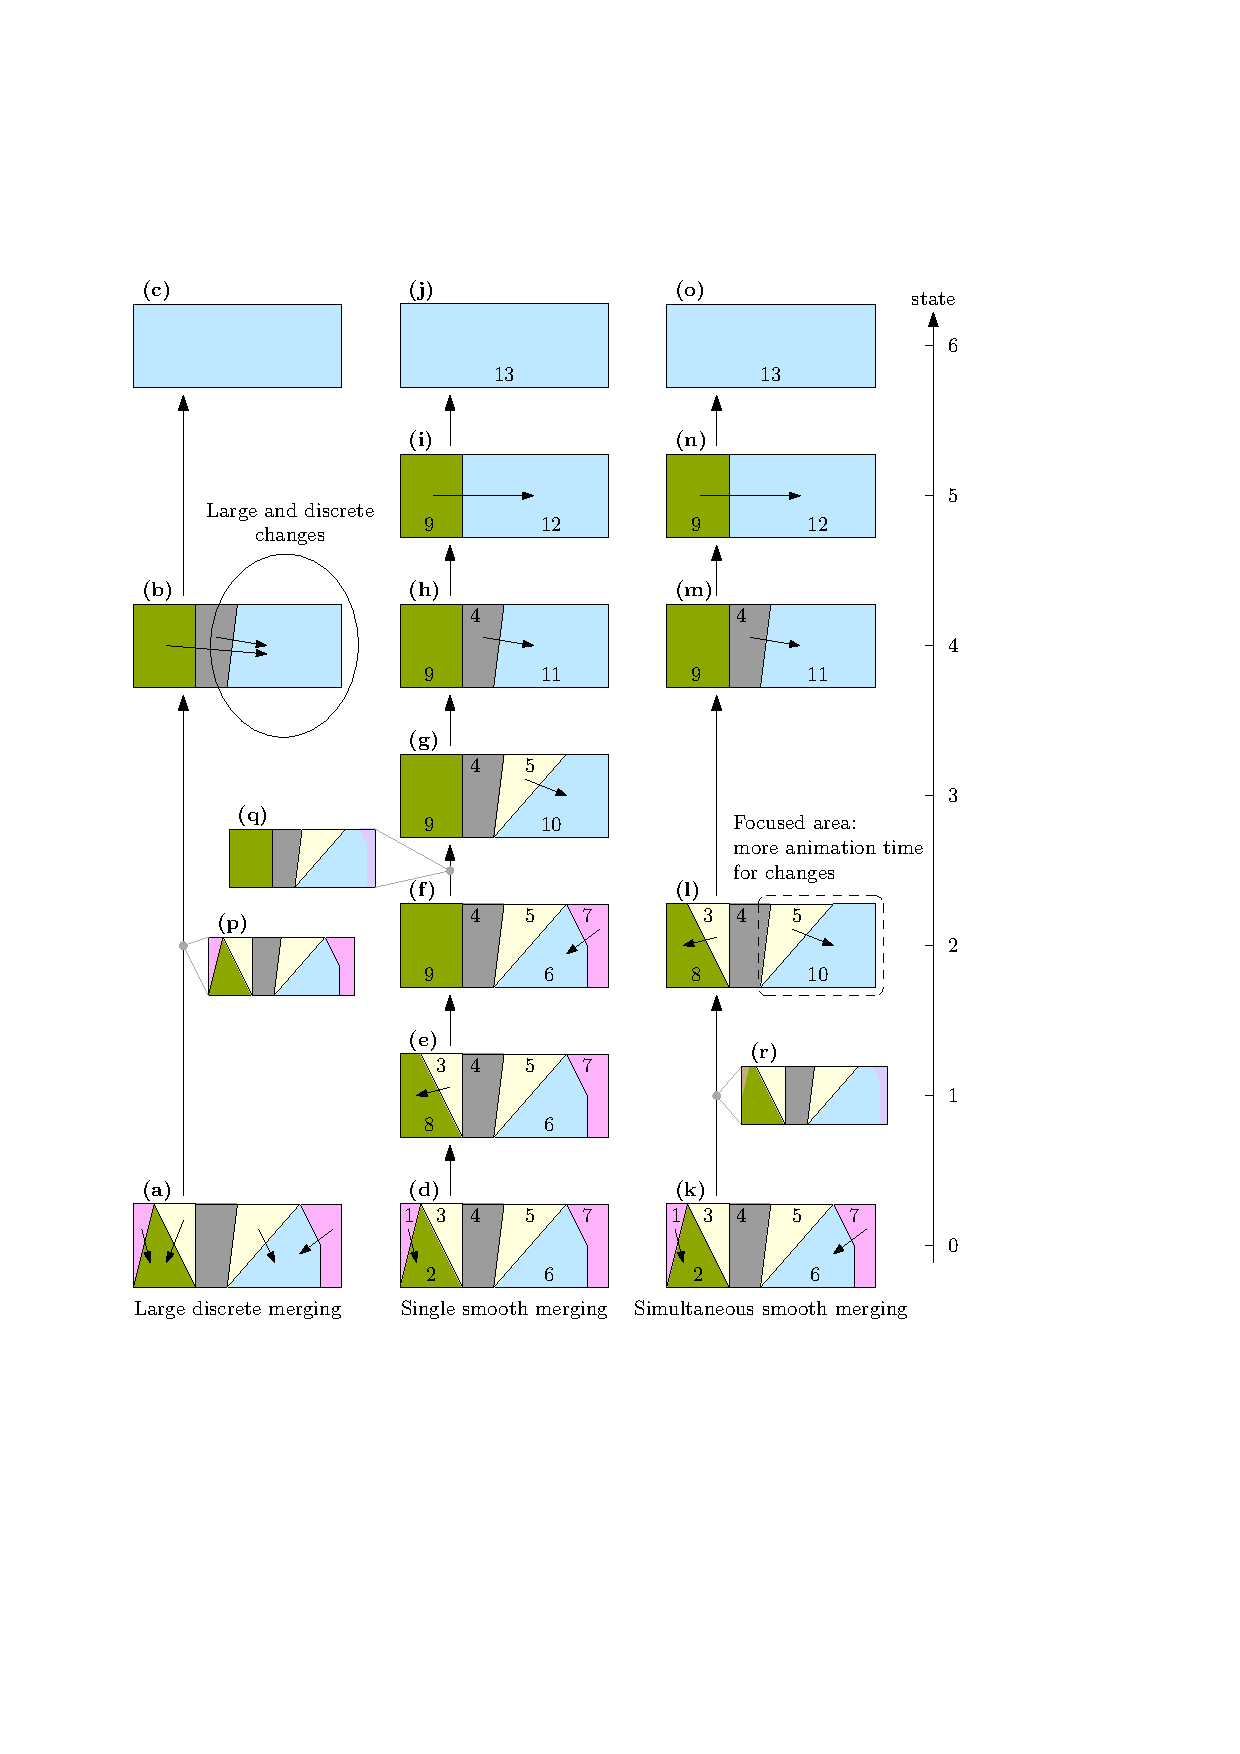
\includegraphics[page=1,width=\linewidth]{introduction}
\caption{The principle of the Eater;
taken from \citet{Suba2014Merge}.}
\label{fig:eater}
\end{figure}



\subsection{Merging considering semantic properties}

As mentioned in \sect\ref{sec:introduction}, 
each of the area objects has its \emph{semantic property} (\ie~class).
When we merge an area into another area, 
the semantic property of the former is changed to that of the latter.
It is important not to cause too much change for two reasons.
First, the generalized map should resemble the base map.
Second, big changes cause users to lose track of their interested areas.

\Citet{vanOosterom1995Development}'s greedy algorithm repeatedly merges 
the least important area with one of its neighbors.
When choosing the neighbor, the algorithm considers 
the compatibility between the least important area and the neighbor,
where the compatibility can be defined based on the semantic property.
\citet{HaunertWolff2010AreaAgg} defined distances between semantic properties 
and included those distances 
into the cost function of their integer linear program.
\citet{Peng2020AreaAgg} defined the semantic distance 
based on a tree of classes,
which guarantees that the distance is a metric 
(see \fig\ref{fig:class_dis}).   


\begin{figure*}[tb]
\centering
\includegraphics[page=3]{introduction}
\caption{A way of defining distances between the classes;
taken from \citet{Peng2020AreaAgg}.}
\label{fig:class_dis}
\end{figure*}

\Citet[][\sect4.4.3]{vanSmaalen2003} mentioned the class-driven generalization, 
where if the two classes of two area objects are under the same super class,
then the two area objects should be merged, 
and the new area object uses the super class.
\Citet[][\sect4.5]{vanSmaalen2003} suggested that
the merging operation should also consider classes that co-occur spatially.
He proposed the \emph{class adjacency index} to measure 
if two classes are often adjacent;
if so, the two objects, with the two classes, should be aggregated,
and a composite class should be used.



\subsection{Simultaneous generalization operators}


Many methods of CMG naturally apply 
multiple generalization operators simultaneously.
In morphing polylines, the points of the polylines are moved at the same time
\citep[\eg][]{Noellenburg2008,Li2017Annealing}.
\citet{Li2017_Building} simultaneously generalized individual buildings.
\citet{Peng2017Building} and \citet{Touya2017Progressive}
generalized buildings to built-up areas.
However, there is no simple relationship 
between their intermediate-scale maps and their source maps.
Therefore, all the intermediate-scale maps of buildings have to be
sent from the server to the clients,
which is network intensive.



\subsection{Gradual transformation in web environment}

Based on the SSC, \citet{Meijers2020Web} explained the principles of 
implementing a web map of area objects.
They showed how to request only a part of a large dataset of a vario-scale map.
They made chunks of the SSC data
so that they were able to send only the chunks relevant 
to users' interested place.
They showed how to efficiently slice the SSC 
to output a web map at a given scale 
using the GPU at the client side.
In addition to slicing the SSC with a horizontal plane,
they also sliced the SSC with a curly surface 
to have a locally more detailed map
or with a tilted surface to have a perspective view.
\citet{Huang2016Webmap} pointed out that
the effort of implementing online maps 
had been spent mainly on preparing data on the server side.
They studied the communication of map data 
between the server side and the client side.
They proposed different strategies of assigning 
the work of processing map data
according to the machine abilities of the clients
(\ie~thin, medium, or thick client).
Their implementation or \emph{option C}
supports gradual transformation of objects.
For a zooming operation, that implementation
continuously requests data from the server side 
and present them on the map 
until the map of the target scale is complete.
\citet{Peng2020Viewer} presented a tool to compare two web maps side by side.
In order to allow users to easily access other map information,
the tool presents a multi-scale raster layer as the background.
Their example respectively used a vario-scale and a multi-scale 
vector layer as the foregrounds and compared between them.






%\citet{Huang2017Matrix} utilized a matrix to guide 
%both pruning rivers and removing vertices for a river network, 
%where the rows and the columns respectively represent
%the rivers and the vertices.
%According to the matrix, 
%they were able to decide which rivers and vertices 
%should remain for a given scale.
%To that purpose, they proposed a method 
%to compute how many rivers and vertices 
%should be kept according to that given scale.


%\citet{Dumont2020MultiScale}
%\citet{Meijers2015Parallel}


\section{Methodology}
\label{sec:methodology}

\fig\ref{fig:intro} shows three different merging strategies.
In \figs\ref{fig:intro}a1--a3, all the changes 
from a level to the next level are processed in one go,
at a specific point.
In \figs\ref{fig:intro}b1--b7, 
there is only one merging operation from a level to the next level,
and the change is realized by an expanding animation
(see \fig\ref{fig:intro}b8).
In \figs\ref{fig:intro}c1--c5, 
there can be many merging operations from a level to the next level,
and each change is realized by an expanding animation
(see \fig\ref{fig:intro}c6).
The first strategy often brings large and discrete changes
(see for example from a1 to a2),
which should be avoided.
Both the second one and the third one 
have the ability to provide smooth changes.
Comparing to the second strategy, 
the third one results in longer animation durations
for some merging operations 
because the changes can share their animation durations.\footnote{%
A comparison of the single merging and the simultaneous merging can be found at 
\url{https://pengdlzn.github.io/webmaps/2021/10/merge/eg-7-comparer-overlay-single-simultaneous.html},
where the swiper can be moved to see the differences of the two maps,
for example, at scale $1:11{,}832$.}
The smooth changes are realized 
by slicing the space-scale cubes (SSCs) of \fig\ref{fig:ssc}
with a moving horizontal plane.
For example, smooth animations of zooming out are obtained by
slicing an SSC from bottom to top.
In detail, \fig\ref{fig:intro}b8 is obtained by slicing
\fig\ref{fig:ssc}a at~$z= 50$.
The details of slicing an SSC are illustrated in \citet{Meijers2020Web}.
The SSCs of \fig\ref{fig:ssc} were built 
based on the \emph{Eater} of \citet{Suba2014Merge}.
The content of an SSC is stored in an OBJ file,
and the OBJ file can be visualized by software ParaView
(see \fig\ref{fig:ssc}).
In \fig\ref{fig:ssc}, the $z$-coordinates are $100$ times of
the state values in \fig\ref{fig:intro}.
We performed this multiplication for illustrative purpose only, 
where the contents of the SSC in the figures can be better observed.

The SSCs of \fig\ref{fig:ssc}a and \fig\ref{fig:ssc}b respectively 
serve for the single smooth merging 
(\figs\ref{fig:intro}b1--\ref{fig:intro}b7) 
and the simultaneous smooth merging 
(\figs\ref{fig:intro}c1--\ref{fig:intro}c5).
\mine{The differences of the two SSCs result in 
the two different merging processes.
For example, at $z=50$ of \fig\ref{fig:ssc}a, 
there is only one polyhedron with the tilted face,
hence there is only a pair of polygons merging in \fig\ref{fig:intro}b8.
In comparison, there are two polyhedra
with tilted faces at $z=50$ of \fig\ref{fig:ssc}b,
and there are two pairs of polygons merging in \fig\ref{fig:intro}c6.}
Note that the choices of selecting areas to merge 
are made in a pre-processing step and are stored in a database, 
before users start zooming on the map.
Therefore, the choices are independent of users' area objects of interest.



%Our strategy of presenting the static boundary (\ie~the exterior one) 
%is that we store the polylines and 
%draw them with width, 
%where the width is computed according to the map scale on the fly.
%We do not draw the common boundary of 
%a pair of areas that are being merged
%so that it is easy for map users 
%to identify the pairs of areas in transition. 



\begin{figure*}[tb]
\centering
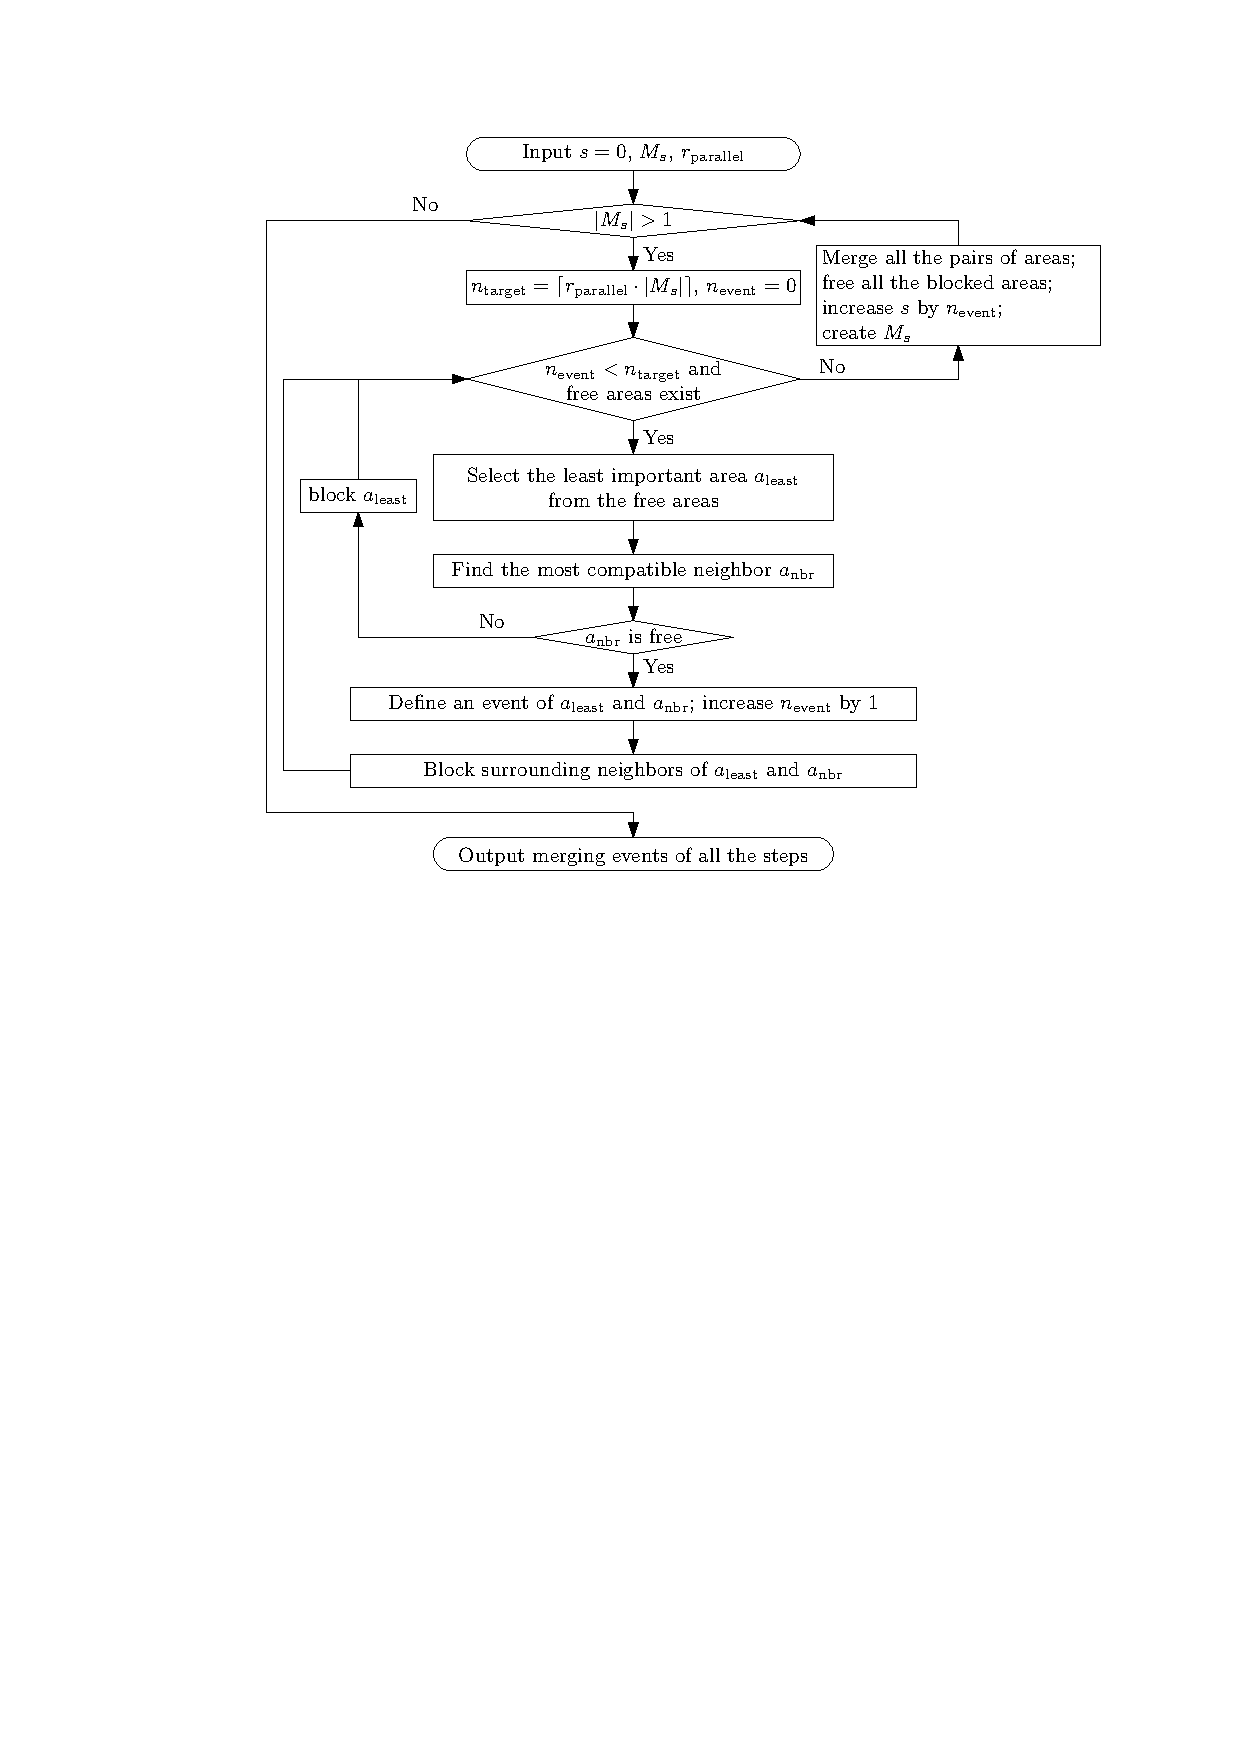
\includegraphics[page=1,scale=0.99]{methodology}
\caption{A comparison of different scale-transition strategies.
Each arrow inside the subfigures indicates a merging operation.
The arrow in the right-hand side indicates the states of zooming out.
%
Subfigures (a1--a3), (b1--b7), and (c1--c5) represent the states
at which the zooming may stop.
Subfigures~(a4), (b8), (c6), and (c7) 
are the map representations during the scale transition,
where their corresponding states are indicated by the gray dots.
The numbers are the IDs of the areas. 
Note that the colors of the smaller areas
adapt to the colors of the larger areas during merging.
}
\label{fig:intro}
\end{figure*}

\begin{figure*}
\centering
\begin{subfigure}[t]{0.48\textwidth}
\centering
\includegraphics[page=2,width=0.95\linewidth]{methodology}
\caption{The SSC of the single merging of \figs\ref{fig:intro}b1--b7.}
\end{subfigure}
\hfill
\begin{subfigure}[t]{0.48\textwidth}
\centering
\includegraphics[page=3,width=0.95\linewidth]{methodology}
\caption{The SSC of the simultaneous merging of \figs\ref{fig:intro}c1--c5}
\end{subfigure}
\caption{
In the left SSC, only one merging event is happening 
at a specific state ($z$-dimension), 
while in the right SSC multiple merging events may happen at the same state.
}
\label{fig:ssc}
\end{figure*}



We define an \emph{event} as a single generalization operation, 
such as merging an area with a neighbor.
For example, \fig\ref{fig:intro}b2 is obtained from 
\fig\ref{fig:intro}b1 by processing one merging event.
Similarly, \fig\ref{fig:intro}c2 is obtained from 
\fig\ref{fig:intro}c1 by processing two merging events.
Note that two areas are neighbors if 
they share a common boundary with length larger than 0
(sharing a point does not make the two areas neighbors).
We define a \emph{step} as 
a set of events happening at the same animation duration,
for example, from \fig\ref{fig:intro}b1 to b2 or
from \fig\ref{fig:intro}c1 to c2.
In our method, a step is completely processed 
before the next step takes place (all sequential).
We define a \emph{state} as the point when a step starts or finishes.
For example, there are seven states 
in the merging sequence of \figs\ref{fig:intro}b1--b7
and five states in the merging sequence of \figs\ref{fig:intro}c1--c5 
(\ie~states 0, 2, 4, 5, and 6).
Note that the value of a state is also 
the total number of events processed so far.


There are two benefits of merging simultaneously.
First, the simultaneity avoids unnatural zooming.
Without the simultaneity,
generalization operations that are processed all sequentially 
may result in no change at some locations in a zooming duration, 
which is unnatural \citep{vanOosterom2014Support}. 
Therefore, \citet{vanOosterom2014Support} 
suggested processing the generalization operations simultaneously,
but no implementation, testing, or assessment of the idea was provided.
Second, the simultaneity brings smoother zooming.
When showing an animation zooming, 
we set $16$ as the default value of the frames per second (FPS).
This value is adequate to provide the visual continuity
\citep[\p24]{Read2000Film}.
If the merging operations happen sequentially instead of simultaneously,
it is more likely that
the time interval between two frames is larger than that between two states.
Then there is no animation of smooth merging shown at all.
For example, if the consecutive frames are 
\figs\ref{fig:intro}b1, \ref{fig:intro}b2, and \ref{fig:intro}b3,
then users can only see discrete merging.
In contrast, if the consecutive frames are 
\figs\ref{fig:intro}c1, \ref{fig:intro}c7, and \ref{fig:intro}c2,
then users can see one frame of ongoing expansion. 
As a result, the merging expansions are visually smoother 
when there are more merging operations processed simultaneously.

When merging simultaneously,
we require that 
the area objects involved in different merging events of the same step 
must not be neighbors.
This requirement makes the merging events independent from each other.
In this way, it is easy for us to maintain the topology of the map.
%Second, users can keep track of their area objects of interest more easily
%than merging several areas into a single one.
In order to realize the requirement,
we \emph{block} the pair of areas of a merging event,
as well as their neighbors.
These areas become \emph{blocked areas}.
The areas are \emph{free} 
if they are not blocked yet.
We develop a greedy algorithm 
to find the simultaneous merging events for each step
in \sect\ref{sec:greedy_algo}.
Then, we integrate the events into the tGAP database tables
(\sect\ref{sec:integrate_tgap}),
followed by integrating the events into the SSC 
(\sect\ref{sec:integrate_ssc}).
In \sect\ref{sec:snap}, we show how to snap the zooming to some valid states
to avoid that the merging animation stops half-way.
In \sect\ref{sec:zooming_duration}, we define 
the animation duration of zooming from one state to another state.
Note that the steps of \sects\ref{sec:greedy_algo}, 
\ref{sec:integrate_tgap}, and \ref{sec:integrate_ssc}  
are done in a preprocess, and the final results are saved in files.
Then the files are sent to the client on request
when a user is browsing the map,
where the steps of \sects\ref{sec:snap} and \ref{sec:zooming_duration}
are done in real time.


\subsection{A greedy algorithm}
\label{sec:greedy_algo}

We use a greedy algorithm 
to find the simultaneous merging events for all the steps.
The merging events will be stored as records in the tGAP database tables
(see \fig\ref{fig:uml_tgap}).
Some instances of the tables are shown in 
\tabl\ref{tbl:face_tgap} of \sect\ref{sec:integrate_tgap}.
To compose a merging event, we wish to
merge the least important area into its most compatible neighbor.
We define the importance and the compatibility according to
\citet{vanPutten1998NewGAP}.
That is, the importance of an area is the multiplication 
of its size and its class weight.
Currently, all the class weights are set to 1,
which leads to that the smallest area is the least important.
The compatibility value between a pair of areas is 
the multiplication of the common boundary's length and 
the class similarity of the two areas.
\appx\ref{appx:create_tables} shows our implementation of
computing the weight values and the class similarities.



\begin{figure*}[tb]
\centering
\includegraphics[page=6]{methodology}
\caption{The Unified Modeling Language (UML) diagram of the classes 
stored in tGAP database tables.
This diagram is a slightly-improved version of 
\citet[\p159]{Meijers2011Thesis}.
In the face table, property \emph{pip\_geometry} 
stores a point (usually the center) in the face (polygon).
The geometry of a face can be obtained 
by calling function \emph{getGeometry()}.
The face geometry is not stored 
because we want to avoid redundancy,
as the edges already stores the sequences of the points.
}
\label{fig:uml_tgap}
\end{figure*}


\fig\ref{fig:greedy_framework} shows the flowchart of our greedy algorithm.
\mine{The process starts with a detailed map of area objects.
The map is denoted by $M_s$, where state~$s$ is 0 at this point.}
Parameter $r_\mathrm{simul}$ specifies 
the proportion (\ie~percentage, when multiplied by~$100$) of area objects that
are expected to be merged simultaneously.
As a value of percentage, 
$r_\mathrm{simul}$ is in the range from~$0\%$ to~$100\%$,
which means~$r_\mathrm{simul} \in [0,1]$.
\mine{We denote by~$|M_s|$ the number of $M_s$'s area objects.}
If there is more than one area ($|M_s|>1$),
then the algorithm finds merging events \mine{for a new step.
In other words, in each iteration when we have $|M_s|>1$,
a set of merging event for a step will be defined.}
We first compute the number of areas that we expect to merge by
\begin{equation}
\label{eq:n_target}
n_\mathrm{target} =
\lceil r_\mathrm{simul} \cdot |M_s| \rceil,
\end{equation}
where \mine{expression $\lceil x \rceil$ returns the ceiling of $x$,
which is the smallest integer greater than or equal to $x$.}
The ceiling function guarantees~$n_\mathrm{target}\ge 1$.
That is to say, the greedy algorithm 
finds at least one merging event for each step.
When $n_\mathrm{target} > 1$, however,
the greedy algorithm cannot always find~$n_\mathrm{target}$ merging events
because some areas may be blocked
(also see \fig\ref{fig:blocked_polygons}).
Therefore, we use variable $n_\mathrm{event}$
to represent the number of events that are actually found for a step. 


\begin{figure*}[tb]
\centering
\includegraphics[page=4]{methodology}
\caption{The flowchart of our greedy algorithm.
\mine{This algorithm finds the merging event for all the steps.
The dashed rectangle marks the process of
finding merging events for a single step.}
}
\label{fig:greedy_framework}
\end{figure*}


\begin{figure*}[tb]
\centering
\includegraphics[page=5]{methodology}
\caption{The process of finding simultaneous merging events for a single step.
    (a) From all the free areas,
	the least important one is selected to merge into
	its most compatible neighbor.
	Then, \mine{the two areas and} the surrounding areas are blocked 
	(marked by the crosses).
	(b) Next, the least important area from the remaining free areas
	is selected to merge with its most compatible neighbor,
	and the relevant areas are also blocked.
}
\label{fig:blocked_polygons}
\end{figure*}

In \fig\ref{fig:greedy_framework},
the dashed rectangle marks the process of 
finding merging events for a single step.
If the process has not found $n_\mathrm{target}$ events yet
($n_\mathrm{event} < n_\mathrm{target}$)
and there are still free areas,
then the process continues looking for merging events.
In detail, the greedy algorithm selects the least important area, 
$a_\mathrm{least}$, from the free areas.
Then, the algorithm finds $a_\mathrm{least}$'s 
most compatible neighbor~$a_\mathrm{nbr}$.
\begin{itemize}[noitemsep,topsep=0pt]
\item If area~$a_\mathrm{nbr}$ is also free, 
a merging event has been found,
consisting of areas~$a_\mathrm{least}$ and~$a_\mathrm{nbr}$.
Consequently, the number of events, $n_\mathrm{event}$, increases by 1.
\mine{Then, $a_\mathrm{least}$, $a_\mathrm{nbr}$, and their neighbors are blocked}
(see \fig\ref{fig:blocked_polygons}a).
Note that if an area shares only one vertex 
with $a_\mathrm{least}$ and/or $a_\mathrm{nbr}$, it is not blocked.
\item If area~$a_\mathrm{nbr}$ is not free,
then it must have been blocked because of the previously found events.
In this case, we block~$a_\mathrm{least}$ for now
so that areas~$a_\mathrm{least}$ and~$a_\mathrm{nbr}$ 
may merge in the next step.
\end{itemize}


\mine{Now, let us move back to the start of
finding merging events for a single step, that is,
the condition ``$n_\mathrm{event} < n_\mathrm{target}$ and
free areas exist''.}
If we have found~$n_\mathrm{target}$ events 
or there is no free area anymore,
then finding merging events of the step finishes.
The greedy algorithm merges all the pairs of areas of the found events
to generate new areas,
frees all the blocked areas,
increases state~$s$ by value~$n_\mathrm{event}$,
and creates map~$M_s$ based on the new areas and the freed areas.
Then, finding merging events for the next step starts.
This loop of finding completes 
when there is only one area left on the map ($|M_s|=1$).
\figs\ref{fig:intro}c1--c5 show a sequence of four merging steps
obtained by our greedy algorithm,
where simultaneous parameter~$r_\mathrm{simul}$ is set to~$0.3$
(Note that this is an extremely high value, 
used here to explain the principle in an artificial simple example).


The ideal situation to apply our method is that 
small areas distribute evenly and the areas do not have holes.
The reason is as follows.
We wish to use a rather large simultaneous parameter~$r_\mathrm{simul}$
so that many events can share their merging durations.
However, if the small areas do not distribute evenly,
then some small areas will be blocked and kept 
while some larger areas will be merged,
which is unreasonable.
If an area has many holes, where each hole is filled with an area, 
then each step a hole merging into its surrounding area will forbid
other holes to merge into it.
This situation results in that 
some holes are merged until the scale is very small.
A typical example is that 
a built-up area contains many buildings as holes.


\subsection{Integrating the simultaneous events into the tGAP database tables}
\label{sec:integrate_tgap}

\citet[\p159]{Meijers2011Thesis} designed three tables 
to record the information of
faces, edges, and face hierarchies, 
which together form a tGAP
\mine{(see \fig\ref{fig:uml_tgap} the UML diagram of the tables)}.
\mine{Note that both class Face and class Edge inherit
 the attributes from superclass tGAPTopolObject.}
The face table contains columns \emph{face\_id}, 
\emph{imp\_low}, \emph{imp\_high}, \emph{imp\_own},
\emph{feature\_class}, \emph{area}, and \emph{mbr\_geometry}.
We add columns \emph{state\_low} ($s_\mathrm{low}$) 
and \emph{state\_high} ($s_\mathrm{high}$) into the table 
so that it is easy to see when a face (\ie~an area object) 
should appear or disappear 
(the same is done also for the edge table).
The values of $s_\mathrm{low}$ and $s_\mathrm{high}$
are assigned when all the pairs of areas are merged
(see the step in \fig\ref{fig:greedy_framework}).
In detail, all those pairs of areas that are merged have 
$s_\mathrm{high} = s + n_\mathrm{event}$,
and the generated areas will have 
$s_\mathrm{low} = s + n_\mathrm{event}$.
\tabls\ref{tbl:face_tgap}a and~\ref{tbl:face_tgap}b 
shows the two new columns with column face\_id.
A face appears as a result of merging two faces during zooming out 
when the slicing arrives at the face's low state.
When the slicing arrives at its high state,
the face should have been merged with another area.
Comparing between the tables of single merging 
(\figs\ref{fig:intro}b1--b7)
and simultaneous merging (\figs\ref{fig:intro}c1--c5),
we observe some differences of the values.
For example, the $s_\mathrm{high}$ values of faces~1 and~2 
are changed from~1 to~2 (see \tabl\ref{tbl:face_tgap}).
Correspondingly, the $s_\mathrm{low}$ value of face~8 is changed from~1 to~2
(see \tabl\ref{tbl:face_tgap}).
Note that the face ids are defined in \fig\ref{fig:intro}.
Similarly to the face tables, 
the columns and records of both the edge table and the face-hierarchy table 
will be changed accordingly.


\begin{table*}[tb]
\caption{Some columns of the face tables. 
    Columns~$s_\mathrm{low}$, $s_\mathrm{merge}$, 
    and~$s_\mathrm{high}$ show the states 
    when the faces appear, when the faces start to disappear, and
    when the faces completely disappear.    
    In table~(b), the different values from table~(a) are underlined.
    Column~$s_\mathrm{merge}$ is not really stored in the database.
    We show the column so that it is easy to see the differences 
    between the $s_\mathrm{low}$ values and the $s_\mathrm{merge}$ values.
    }
\label{tbl:face_tgap}
\begin{subtable}{0.48\textwidth}
\caption{The face table of the single merging 
    shown in \figs\ref{fig:intro}b1--b7.}
\centering
\begin{tabular}{cccc}
\toprule
$f_\mathrm{id}$& $s_\mathrm{low}$    & $s_\mathrm{merge}$ 
& $s_\mathrm{high}$ \\ \midrule
% id         s_low         s_merge         s_high
1       &     0         &     0         &     1       \\
2       &     0         &     0         &     1       \\
3       &     0         &     1         &     2       \\ 
4       &     0         &     4         &     5       \\
5       &     0         &     3         &     4       \\
6       &     0         &     2         &     3       \\         
7       &     0         &     2         &     3       \\
8       &     1         &     1         &     2       \\
9       &     2         &     5         &     6       \\         
10      &     3         &     3         &     4       \\
11      &     4         &     4         &     5       \\ 
12      &     5         &     5         &     6       \\ 
13      &     6         &    ---        &    ---      \\
\bottomrule
\end{tabular}
\end{subtable}
%
\hfill
%
\begin{subtable}{0.48\textwidth}
\caption{The face table of the simultaneous merging 
    shown in \figs\ref{fig:intro}c1--c7.}
\centering
\begin{tabular}{cccc} %\underbar{2}
\toprule
$f_\mathrm{id}$ & $s_\mathrm{low}$   & $s_\mathrm{merge}$ 
& $s_\mathrm{high}$ \\ \midrule
% id         s_low         s_merge        s_high
1       &     0         &     0         &\underbar{2} \\
2       &     0         &     0         &\underbar{2} \\
3       &     0         & \underbar{2}  &\underbar{4} \\ 
4       &     0         &     4         &     5       \\
5       &     0         & \underbar{2}  &     4       \\
6       &     0         & \underbar{0}  &\underbar{2} \\         
7       &     0         & \underbar{0}  &\underbar{2} \\
8       & \underbar{2}  & \underbar{2}  &\underbar{4} \\
9       & \underbar{4}  &     5         &\underbar{6} \\         
10      & \underbar{2}  & \underbar{2}  &\underbar{4} \\
11      &     4         &     4         &     5       \\ 
12      &     5         &     5         &     6       \\ 
13      &     6         &    ---        &    ---      \\
\bottomrule
\end{tabular}
\end{subtable}
\end{table*}


\subsection{Integrating the simultaneous events into the SSC}
\label{sec:integrate_ssc}

Recall that we merge a pair of areas by expanding
the winner over the loser.
The Eater of \citet{Suba2014Merge} is used to 
triangulate the loser and to tilt the triangles.
Then, the tilted triangles are integrated into the SSC
(see \fig\ref{fig:ssc})
so that we can slice the SSC to achieve smooth merging.
For the case of single merging,
if a pair of areas have state-high value~$s_\mathrm{high}$,
then the merging animation 
always starts at state~$s_\mathrm{merge}=s_\mathrm{high}-1$
(see \tabl\ref{tbl:face_tgap}a).
The less important area completely disappears
at state~$s_\mathrm{high}$.
In the face table, a row will be added to record the new area, 
and its $s_\mathrm{low}$ value 
will be the previous~$s_\mathrm{high}$ value.
The new area takes over the combined place of the pair of areas.
Take \fig\ref{fig:intro} as an example, 
area~1 is merged into area~2 (\fig\ref{fig:intro}b1), 
and area~8 is generated to take over the combined place (\fig\ref{fig:intro}b2).
The tilted triangle is the one that spans 
from~$z= 0$ to~$z=100$
in \fig\ref{fig:ssc}a.
In \tabl\ref{tbl:face_tgap}a, 
the~$s_\mathrm{low}$ value of area~8 is 1,
which is the~$s_\mathrm{high}$ value of areas~1 and~2.

For the case of simultaneous merging,
if a step consists of~$n_\mathrm{event}$ events and 
the step finishes at state~$s_\mathrm{high}$, then the step starts 
at state~$s_\mathrm{merge}=s_\mathrm{high} - n_\mathrm{event}$.
The reason is that if the~$n_\mathrm{event}$ events 
would happen sequentially (\ie~single merging),
then the first of the $n_\mathrm{event}$ events would start at
state~$s_\mathrm{high} - n_\mathrm{event}$,
the second would start at
state~$s_\mathrm{high} - n_\mathrm{event} + 1$, and so on.
Now that all the~$n_\mathrm{event}$ events share their merging durations,
all of them can start at state~$s_\mathrm{high} - n_\mathrm{event}$.
As a result,
each of the simultaneous events has more time to take place
than the events would happen sequentially.
In other words, for a merging step,
each of the events has more time to take place 
if there are more simultaneous events.

In order to build the SSC for simultaneous merging,
we need the~$s_\mathrm{merge}$ value for each of the merging steps
so that we know from which state 
the triangles of loser's ceiling should be tilted.
A simple way is to add a column, say, $s_\mathrm{merge}$
into the face table during generating the tGAP, 
as done in \tabl\ref{tbl:face_tgap}.
Then, the states of starting merging can be recorded into the column.
However, we would like to avoid unnecessary columns to save storage.
Therefore, we compute~$s_\mathrm{merge}$ values 
based on the~$s_\mathrm{high}$ values
on the fly when building the SSC.
As an event involves two areas,
the number of events finishing at state~$s_\mathrm{high}$ 
can be calculated by:
\begin{equation}
\label{eq:n_event_state}
n_\mathrm{event} (s_\mathrm{high}, \mathrm{\textbf{s}_{high}}) = 
\frac{\sum\limits_{s \in \mathrm{\textbf{s}_{high}}} \{s=s_\mathrm{high}\}}{2}
\end{equation}
where vector~$\mathrm{\textbf{s}_{high}}$ 
denotes the values
recorded in column~$s_\mathrm{high}$ of the face table
(\eg~\tabl\ref{tbl:face_tgap}b).
Expression~$\{s=s_\mathrm{high}\}$ returns~$1$ if the two values are equal 
and returns~$0$ otherwise.
As illustrated before, the state at which the simultaneous merging starts 
can be computed by:
\begin{equation}
\label{eq:s_merge_state}
s_\mathrm{merge} (s_\mathrm{high}, \mathrm{\textbf{s}_{high}}) = 
    s_\mathrm{high} - 
    n_\mathrm{event} (s_\mathrm{high}, \mathrm{\textbf{s}_{high}})
\end{equation}



Take the case of \tabl\ref{tbl:face_tgap}b for example,
we have~$\mathrm{\textbf{s}_{high}} 
= [2, 2, 4, 5, 4, 2, 2, 4, 6, 4, 5, 6]$, 
$n_\mathrm{event} (4, \mathrm{\textbf{s}_{high}}) = 2$, 
and $s_\mathrm{merge} (4, \mathrm{\textbf{s}_{high}}) = 2$.
Therefore, there are two merging events finishing at state~$4$,
\ie~the event of merging area 3 into area~8 and 
the event of merging area~5 into area~10 
(also see \figs\ref{fig:intro}c2 and~\ref{fig:intro}c3).
The merging animation takes place from state~$2$ to state~$4$.
This merging can also be observed from 
the two tilted triangles spanning from~$z = 200$ to~$z = 400$ 
in \fig\ref{fig:ssc}b.
In merging sequence of \figs\ref{fig:intro}b1--b7, 
the animation of merging area~3 into area~8 
takes place from state~$1$ to state~$2$
(also see the tilted triangle spanning from~$z = 100$ to~$z = 200$ 
in \fig\ref{fig:ssc}a), and 
the animation of merging area~5 into area~10
takes place from state~$3$ to state~$4$
(also see the tilted triangle spanning from~$z = 300$ to~$z = 400$ 
in \fig\ref{fig:ssc}a).
As a result, the animation duration of merging area~3 into area~8 of 
sequence \figs\ref{fig:intro}c1--c5
is almost twice as that of sequence \figs\ref{fig:intro}b1--b7.
We say \emph{almost} because the animation duration is also dependent on 
the state value of the map
(see \sect\ref{sec:zooming_duration}).


\subsection{Snapping to a valid state}
\label{sec:snap}

For a zooming action based on the SSC, 
we always snap the map to a valid state.
In this way, users will not see a merging operation stopping half-way.
Take the sequence of \figs\ref{fig:intro}c1--c5 for example, 
the merging animation is allowed to stop at 
\ref{fig:intro}c1 or \ref{fig:intro}c2,
but not at \ref{fig:intro}c6 or \ref{fig:intro}c7.
In this example, state~$1$ is invalid
because some merging operations have not completed.
Here, the list of valid states 
is~$\mathrm{\textbf{s}_{valid}} = [0, 2, 4, 5, 6]$.
In order to snap to one of the valid states,
we have to communicate them to the client side. 
There are multiple options. 
The simplest one assumes that, 
the greedy algorithm can always find
the~$n_\mathrm{target}$ number of events in all steps. 
In that case, we just need to communicate 
the number of areas and the ratio~$r_\mathrm{simul}$. 
However, this assumption may be incorrect in case of high value ratios (\eg~$r_\mathrm{simul} > 0.01$). 
We then have to communicate the valid states by sending them explicitly. 
Because this list may get rather large,
we only send exceptions 
(see \appx\ref{appx:communicate_valid_states} for more details).
As a result, the list of valid states~$\mathrm{\textbf{s}_{valid}}$ 
is generated on the client side.


According to how much a user has zoomed,
the target scale, say, $1:S_\mathrm{t}$ can be computed.
\citet{Huang2016Webmap} suggested that 
the average density of the base map should be preserved 
for a smaller-scale map.
Their suggestion is based on the assumption that 
the area density of the base map is well designed, which is reasonable.
We use variable~$A_\mathrm{real}$ to denote the total areal size of 
all the area objects in reality.
Then, the size on screen at scale~$1:S_\mathrm{t}$ 
is~$A_\mathrm{real} \big/ S^2_\mathrm{t}$.
In order to keep the density, we require
\begin{equation}
\label{eq:equal_density}
\frac{N_\mathrm{b}}{A_\mathrm{real} \big/ S^2_\mathrm{b}} =
\frac{N_\mathrm{b}-E_\mathrm{t}}{A_\mathrm{real} \big/ S^2_\mathrm{t}}
\end{equation}
where parameter~$N_\mathrm{b} = |M_0|$ 
is the number of areas on the base map,
parameter~$S_\mathrm{b}$ is the scale denominator of the base map,
and variable~$E_\mathrm{t}$ is the total number of events 
processed from the base map to the map at scale~$1:S_\mathrm{t}$
(in this case, an event is that an area is merged into another one).
\eq\ref{eq:equal_density} yields:
\begin{equation}
\label{eq:E_t}
E_\mathrm{t} = N_\mathrm{b} \left(1-\frac{S^2_\mathrm{b}}{S^2_\mathrm{t}}\right)
\end{equation}
In our example of \figs\ref{fig:intro}c1--c5,
if event number~$E_\mathrm{t} \le 0$, the base map should be presented;
if $E_\mathrm{t} \ge 6$,
the map with the final single area should be presented.
Otherwise, if $0<E_\mathrm{t} < 6$, we snap event number~$E_\mathrm{t}$ 
to a value (measured in events) of 
list~$\mathrm{\textbf{s}_{valid}}$,
which is denoted by~$E_\mathrm{t,snap}$.
The snapping also depends on if the map user is zooming in or out.
For zooming in, $E_\mathrm{t,snap}$ 
is the closest value in $\mathrm{\textbf{s}_{valid}}$ that is 
smaller than or equal to $E_\mathrm{t}$.
For zooming out, $E_\mathrm{t,snap}$ 
is the closest value in $\mathrm{\textbf{s}_{valid}}$ that is 
larger than or equal to $E_\mathrm{t}$.
This way of snapping prevents $E_\mathrm{t,snap}$ from
being the same value before zooming;
otherwise, the map will stand still 
if the map user zooms only a little bit.
The scale denominator corresponding to event number~$E_\mathrm{t,snap}$
can be computed by 
\begin{equation}
\label{eq:S_t_snap}
S_\mathrm{t,snap} = S_\mathrm{b} \sqrt{\frac{N_\mathrm{b}}{N_\mathrm{b}-E_\mathrm{t,snap}}}
\end{equation}
where this equation is an inverse function of \eq\ref{eq:E_t}.
At the end of the zooming action, 
the map will snap to state~$s_\mathrm{t,snap}$
at scale~$1:S_\mathrm{t,snap}$.
Note that state~$s_\mathrm{t,snap}$ always has 
the same value as event number~$E_\mathrm{t,snap}$.



\subsection{Animation duration of a step}
\label{sec:zooming_duration}

When users are zooming from a scale to another scale,
some steps take place to change the state of the map accordingly.
We define the \emph{zooming duration} as the amount of 
animation time that the map reacts to one ``rolling click'' of the mouse wheel.
The zooming duration often is the sum of 
the \emph{animation durations} of several merging steps.
The animation duration of each event depends on 
the number of events between the two states,
the \emph{zooming factor} of the scale, and 
the \emph{zooming duration}.
On the one hand, the animation duration should not be too short 
as then the animation will be too fast. 
On the other hand, if the animation takes too long, 
the map will not be interactive, and users will be ``frustrated''.
\citet[][\sect4.3]{Meijers2020Web} 
have introduced the zooming factor and the zooming duration.
They allowed users to set the two parameters,
which is also the case in our paper
(see \fig\ref{fig:interaction_settings}).
This section formalizes the relationship of the animation duration,
the zooming duration, the zooming factor, and the number of events.
In a zooming duration, there can be many merging steps,
no matter single merging or simultaneous merging.
The formalization is based on the setting that
a zooming duration is divided equally by its merging steps
(\citet[][\sect6.7]{Suba2017Thesis} showed some other possible settings).
In other words,
the steps happen sequentially and take the same amount of animation duration.
Note that the steps from different zooming durations 
may have different animation durations.

\begin{figure*}[tb]
\centering
\includegraphics[page=7,scale=0.9]{methodology}
\caption{Our panel of settings. 
Among others, one can set how much to zoom when scrolling the mouse wheel 
and set the zooming duration. 
}
\label{fig:interaction_settings}
\end{figure*}

Let $N_\mathrm{event}$ be the number of events happening in a zooming duration.
Let $n_\mathrm{step}$ be the number of steps happening in the zooming duration.
Let $t_\mathrm{single}$ be the animation duration of each of the steps,
where each step consists of only one event.
Let $t_\mathrm{simul}$ be the animation duration of each of the steps,
where each step consists of at least one event.
Then, we have 
\begin{equation}
\label{eq:t_compare}
t_\mathrm{simul} = t_\mathrm{single}  \frac{N_\mathrm{event}}{n_\mathrm{step}}
\end{equation}
As~$N_\mathrm{event}$ is larger than or equal to~$n_\mathrm{step}$,
we have $t_\mathrm{simul} \ge t_\mathrm{single}$.
That is to say, when processing the merging events simultaneously,
each step has more time to take place. 
The derivation of \eq\ref{eq:t_compare} is shown 
in \appx\ref{appx:animation_duration_event}.







\section{Case study}
\label{sec:case_study}


%\textbf{How much data to be loaded?}
%\textbf{How much time for loading data?}


We have stored the result of the tGAP 
as a set of tables (see \sect\ref{sec:integrate_tgap}) 
in a PostgreSQL database.
We have employed the Eater of \citet{Suba2014Merge},
implemented in Python, 
to generate the elements
(vertices, triangulated faces, and boundaries)
of the SSC \citep{vanOosterom2014tGAPSSC} 
and saved these elements in an OBJ file.\footnote{%
Wavefront .obj file:
\url{https://en.wikipedia.org/wiki/Wavefront_.obj_file},
accessed: January 14, 2020.}
When a user visits our website to access the map,
some data will be sent to the client side.  
On the client side,
the received data will be processed
by a map viewer implemented in JavaScript.
The processed data and some code based on WebGL (Web Graphics Library)
are submitted to GPU so that 
the interactive map with smooth zooming
can be output by slicing the SSC.


%
\fig\ref{fig:data} shows the topographic map of this case study.\footnote{%
    \fig\ref{fig:data}a is obtained from article 
    \emph{12 Most Beautiful Regions in the Netherlands}; see
    \url{https://www.touropia.com/regions-in-the-netherlands-map/},
    accessed: October 5, 2021.}
The class codes and the rendering formulas are provided by the Dutch Kadaster.\footnote{%
See the details at
\url{http://register.geostandaarden.nl/visualisatie/top10nl/1.2.0/BRT_TOP10NL_1.2_beschrijving_visualisatie.xlsx},
accessed: January 15, 2020.}
%
Because the base scale is $1:10{,}000$, 
we have~$S_\mathrm{b} = 10{,}000$ for \eq\ref{eq:S_t_snap}.
The maximum value of event number~$E_\mathrm{snap}$ is~$13{,}237$
as there are in total~$13{,}238$ areas.
When we zoom out far enough 
so that~$E_\mathrm{snap}$ reaches its maximum value,
the scale denominator arrives at~$1{,}150{,}565$
according to \eq\ref{eq:S_t_snap}.
At that moment, all the areas are merged into one single area.
In each step, we want to simultaneously merge some proportion of the areas.
We tried three cases: 0.1\%, 1\%, and 10\%.
That is, simultaneous parameter~$r_\mathrm{simul}=0.001, 0.01, \text{and~} 0.1$ 
(see \sect\ref{sec:greedy_algo}), 
which are independent of the size of the map dataset.
\fig\ref{fig:web_map} shows two examples of our web map when 
simultaneous parameter~$r_\mathrm{simul}=0.01$.\footnote{%
The three versions of the map can be browsed online at
\url{https://pengdlzn.github.io/webmaps/2021/10/merge/}.}


\begin{figure}[tb]
\centering
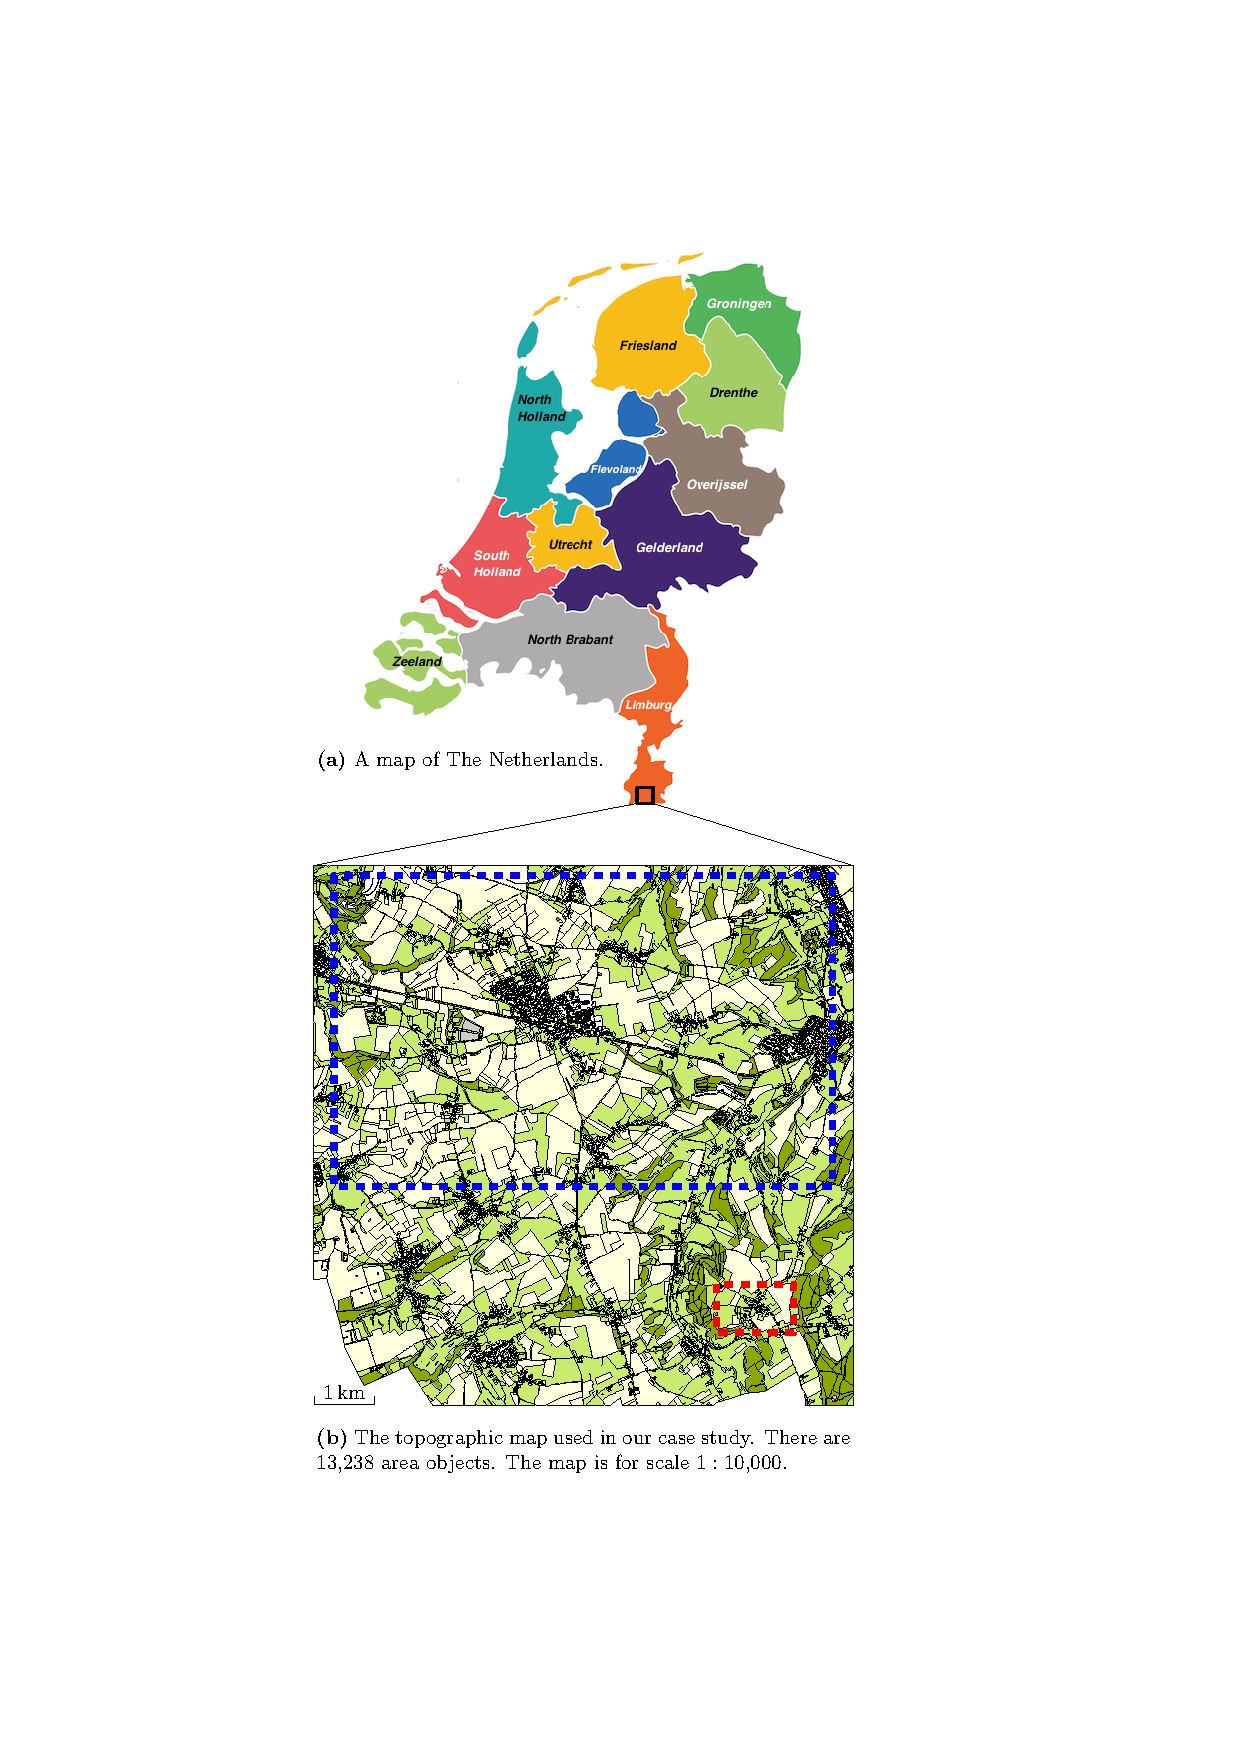
\includegraphics[page=1,draft=false,width=\linewidth]{data}
\caption{The data used in our case study.}
\label{fig:data}
\end{figure}


\begin{figure}[tb]
\centering
\begin{subfigure}[t]{0.49\textwidth}
\centering
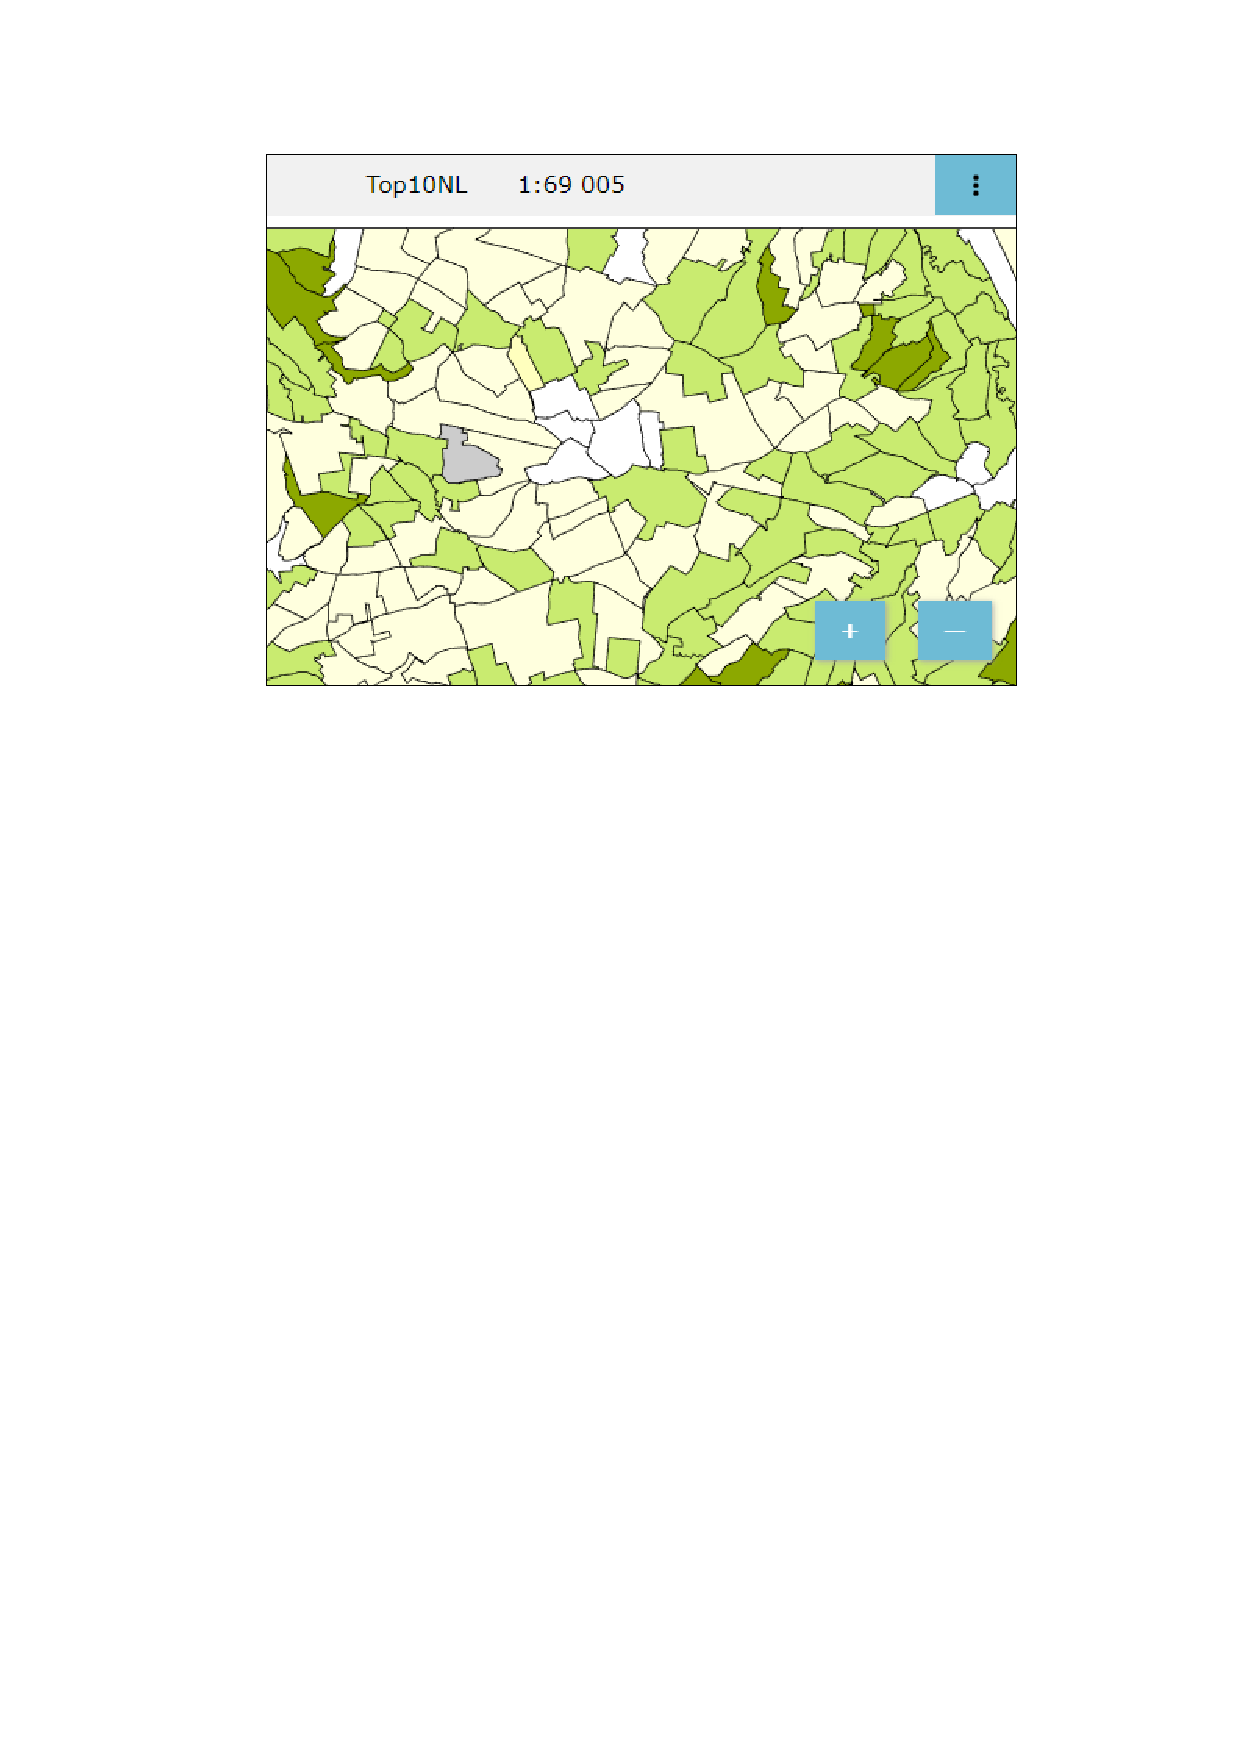
\includegraphics[page=1,scale=0.8]{case_study}
\caption{A part of the base map. The place is marked 
    by the red dashed rectangle in \fig\ref{fig:data}b.}
\end{subfigure}
\newline
\vspace{0.5cm}
%
\begin{subfigure}[t]{0.49\textwidth}
\centering
\includegraphics[page=2,scale=0.8]{case_study}
\caption{An overview map.\mine{The place is marked 
    by the blue dashed rectangle in \fig\ref{fig:data}b.}
   The overview map is generated from the base map 
    by simultaneous merging with parameter~$r_\mathrm{simul}= 0.01$.}
\end{subfigure}
\caption{Two examples of our web map with different scales.
    }
\label{fig:web_map}
\end{figure}

Some statistics of the results when 
simultaneous parameter~$r_\mathrm{simul}=0.001$, $0.01$, or $0.1$ 
are shown in \tabl\ref{tbl:simultaneous_param_comparison}.
According to column~$N_\mathrm{step}$,
the number of steps decreases 
when the simultaneous parameter increases.
This is reasonable because more areas will be merged in each step.
As explained in \sect\ref{sec:greedy_algo}, 
for each merging step we iteratively select the least important area 
and its most compatible neighbor to define a merging event; 
then, we block the two areas and their neighbors.
Sometimes, a least important area is already blocked 
because of the previously found events.
This situation happens~$2{,}714$ times in total for all the steps
when simultaneous parameter~$r_\mathrm{simul}=0.01$
(see column~$N_\mathrm{blocked}$ of 
\tabl\ref{tbl:simultaneous_param_comparison}).
%
Sometimes, although a least important area is free, 
its most compatible neighbor has been blocked 
because of the previously found events.
This case happens~$1{,}383$ times in total for all the steps
when $r_\mathrm{simul}=0.01$
(see column~$n_\mathrm{nbr\_blocked}$ of 
\tabl\ref{tbl:simultaneous_param_comparison}).
%
According to the statistics, we encounter more cases of the areas blocked
when merging a larger proportion of the area objects.
However, we can still reach our target number of events perfectly 
for settings of~$r_\mathrm{simul}=0.01$ or~$r_\mathrm{simul}=0.001$. 
Only when pushing beyond the limit (\eg~$r_\mathrm{simul}=0.1$), 
we can not reach the target number of events in a step 
(and we need correction information 
to compute the actual number of found events). 
When the target number of events cannot be met, 
one could also question the cartographic quality 
because there is hardly any free choice when generalizing.


\begin{table}[tb]
\centering
\caption{Some statistics when different simultaneous parameters area used.
    Column~$N_\mathrm{step}$ records the number of steps to transit 
    from the base map to the map with a single area.    
    Column~$N_\mathrm{blocked}$ records the number of times
    when the least important area was blocked.
    Column~$N_\mathrm{nbr\_blocked}$ records the number of times 
    when the most compatible neighbor was blocked.
}
\begin{tabular}{rrrr}
\toprule
$r_\mathrm{simul}$   & $N_\mathrm{step}$ & $N_\mathrm{blocked}$  & $N_\mathrm{nbr\_blocked}$ \\ \midrule
0.001                   &  3{,}195          &       211             &       72                  \\
0.01                    &  544              &   2{,}714             &  1{,}383                  \\
0.1                     &  91               & 100{,}617             & 34{,}268                  \\ 
\bottomrule 
\end{tabular}
\label{tbl:simultaneous_param_comparison}
\end{table}



As we can find the target numbers of merging events for all the steps
when simultaneous parameter~$r_\mathrm{simul}= 0.001$ or~$0.01$, 
the corresponding exceptions lists are empty.
When~$r_\mathrm{simul}= 0.1$,
the exception list is
$$[[1, 1304], [2, 1070], \dots, [77, 2]],$$
which has~$71$ pairs of values.
In reality, we would not use~$r_\mathrm{simul}= 0.1$
(merging~$10\%$ of the current areas in every step)
because it is an unrealistic high value.
Using such a high value results in a multi-scale representation
(because we have a few valid states or scales),
whereas we would like to have representations at nearly
arbitrary scales.

%Important note: this is for a small subset 9x9 
%out of the 300x300 km^2 (whole country). 
%To have same effect can we keep the r_parellel at same value, 
%but we will have less situation where the target is not reached (more options)


Comparing to the map based on the single merging,
the map based on the simultaneous merging indeed 
provides smoother zooming.
We set zooming factor~$f_\mathrm{zoom}=1$ and 
zooming duration~$t_\mathrm{zoom}=1 s$ 
(see \sect\ref{sec:zooming_duration}).
The map based on the single merging gives the impression
of discrete scale transition, 
where it is difficult to see a winner expands over a loser.\footnote{%
See the web map at
\url{https://pengdlzn.github.io/webmaps/2021/10/merge/limburg-single-merging}.} 
The reason is that the merging happens too fast,
so the time for animation available is too short.
This is also the case when 
we use simultaneous parameter~$r_\mathrm{simul}= 0.001$.\footnote{%
See the web map at
\url{https://pengdlzn.github.io/webmaps/2021/10/merge/limburg-0.001.html}.}
We get the feeling of smooth merging when~$r_\mathrm{simul}= 0.01$.\footnote{%
See the web map at
\url{https://pengdlzn.github.io/webmaps/2021/10/merge/limburg-0.01.html}.}
When~$r_\mathrm{simul}= 0.1$, 
the smooth merging is already obvious.\footnote{%
See the web map at
\url{https://pengdlzn.github.io/webmaps/2021/10/merge/limburg-0.1.html}.}
 



%\begin{figure}[tb]
%\centering
%\includegraphics[page=3,scale=0.8]{case_study}
%\caption{
%    The map to the left of the slider is based on single merging,
%    and the one to the right is based on simultaneous merging
%    with~$r_\mathrm{simul}= 0.1$.
%    The slider can be moved to tune the widths of the two map canvases.
%    The two maps are very different, and 
%    we can observe some sudden changes across the slider.
%}
%\label{fig:comparison}
%\end{figure}

\mine{\fig\ref{fig:problem} shows a problem 
when we use simultaneous parameter $r_\mathrm{simul}= 0.1$.
That is, some tiny and relatively unimportant areas stay 
until the scale is quite small,
where they should be merged when the scale is larger.
This problem has been mentioned in \sect\ref{sec:greedy_algo}.}
The reason of the problem is that 
there are many buildings in the middle of the figure.
When the buildings share the same surrounding area,
they become its holes.
In each step, only one of the buildings can be merged into the surrounding area
because of the blocking.
In the meantime, the areas at other places of the map merge relatively fast
because we except to merge $10\%$ of the areas in each step.
Fortunately, we would not need to 
use such a big simultaneous parameter in reality.


\begin{figure}[tb]
\centering
\includegraphics[page=3,scale=0.8]{case_study}
\caption{
    Some tiny areas should be merged when the scale is larger,
    where the simultaneous parameter is $0.1$.
}
\label{fig:problem}
\end{figure}




\section{Concluding remarks}
\label{sec:concluding_remarks}

\subsection{Conclusion}
%For the first time, 
This paper has examined the simultaneous processing 
of generalization operations,
using the merging operation as a case study. 
The purpose of having simultaneous generalization operations 
is to provide smoother zooming experience later on 
(compared to the pure sequenced individual generalization events)
so that users can better keep track of their interested objects.
This paper developed a greedy algorithm to find simultaneous events of 
merging area objects.
The simultaneous events were integrated into 
the tGAP and the SSC to nicely visualize the merging animations.
To guarantee that the merging animations 
are completely shown while zooming, 
we managed to snap zooming operations to valid states.
This paper also presented a recipe 
to define the animation duration of an event.
According to our case study,
the simultaneous merging indeed provides smoother zooming
than the single merging.




\subsection{Future work}

Many topics related to this research need to be studied further.
Our case study with $13{,}238$ area objects 
demonstrated the efficiency of our prototype.
In our case study, all the data of the SSC is stored in a single file
because the tested map is not very big.
The map will display only after the whole file is loaded.
For a topographic map with much more objects,
we are also developing a method that divides the SSC into many parts, 
and each part is stored in a file.
A file will be dynamically loaded 
when the user is reading the relevant place and scale of the map.
This strategy also allows progressive transfer of data
\citep{vanOosterom2014Support}.
Further, a file at the client side will be removed to release main memory
if the corresponding part of map is not browsed for a long time. 
With those functionalities, our prototype is able to handle 
a map with arbitrary number of area objects.

This paper used a greedy algorithm 
to find simultaneous merging events for each step.
Alternatively, it is possible to define merging steps 
by selecting and combining some single-event steps of a sequence found 
by some existing methods
(\eg~the greedy algorithm of \citet{vanOosterom2005}
or the \Astar algorithm of \citet{Peng2020AreaAgg}).

Currently, the merging events distribute randomly on a map.
If we are unlucky, there may be a lot of events 
happening in users' focused region for a zooming duration,
which may cause the users to lose track of their interested objects;
for another zooming duration, 
there may be no event happening in the focused region at all.
The strategy of blocking neighboring areas in our greedy algorithm 
already mitigates the problem.
However, it may be even better if 
we explicitly distribute the merging events evenly, 
then the workload for a user to follow the events is stable during the zooming.
To this end, we could divide a map into many regions 
using a field-tree-like, multiple-level grid \citep{vanPutten1998NewGAP}
or using the road network.
Then, we could find a certain number of events in each of the regions 
according to the regions' sizes,
which should result in an even distribution of events.
Finally, we could compare our greedy algorithm and 
the algorithm considering even distribution.

Our current event consists of only the merging operation,
it is also necessary to involve split operation
because sometimes a merging operation results in an unnatural area.
For example, it is weird to merge a long and thin area 
with one of the areas that are along it
\citep[see][]{Haunert2008Skeleton}.
Therefore, such kind of long and thin areas should be
split into several parts first.
We may integrate a split method based on the straight skeleton
\citep{Haunert2008Skeleton}
or the skeleton obtained from a CDT
\citep{Ai2002GAP,Meijers2016Split}.
In addition to area features, we also need to support line features 
(\eg~roads, river, rail).
In order to apply appropriate generalization operators
for a certain scale,
we need to extend and implement the framework 
to guide the generalization choices
\citep{Meijers2018Framework}.


To avoid clutter of vertices for zooming out, 
it is necessary to simplify the boundaries of the areas.
Many existing methods could be integrated into our simultaneous paradigm.
\citet{Meijers2011LineSimp} proposed a method 
to simplify the boundaries simultaneously. 
The results are topologically safe. 
Another choice would be the method of \citet{ImaiIri1988},
which is able to minimize the number of vertices 
for a given error threshold.
One more choice would be to construct compatible triangulations 
\citep[see][\chap3]{Peng2019Thesis}
for the two levels of topographic maps.
In the SSC, we could build some tilted walls 
to connect the two levels of compatible triangulations.
When we slice this SSC to animate a zooming action,
the boundaries of the areas are morphed 
(moved smoothly and simultaneously)
between a detailed representation and a coarse representation.


This paper develops the technique for 
smooth zooming based on simultaneous merging,
and we hope that it allows map users to follow the zooming more easily.
A future work is to examine 
how much map users benefit from our technique.
We will conduct some usability tests based on the experience of
\citet[\sect6.7]{Suba2017Thesis} and \citet{Midtbo2007}.
Another future work is to find optimal simultaneous parameters for 
different kinds of datasets.


%Some research questions are as follows.
%What aspects should we optimize 
%(\eg~minimizing the number of merging events or 
%assigning similar numbers of merging steps to each event)?
%What algorithm should we use 
%(\eg~dynamic programming, \Astar, or integer linear programming)?
%How much time is gained for users to observe the merging steps on the screen?
%How to store the simultaneous merging steps?




%\section*{Data and codes availability statement}
%
%The data and codes used in this case study 
%can be found at \emph{figshare} 
%(see \url{https://figshare.com/s/199e049e2a0f9c18d19a}).
%The data was derived from open-access dataset TOP10NL,
%which is a topographic map produced by Kadaster
%(see \url{https://www.pdok.nl/downloads/-/article/basisregistratie-topografie-brt-topnl}).
%\footnote{%
%Dataset TOP10NL can be downloaded at
%\url{https://www.pdok.nl/downloads/-/article/basisregistratie-topografie-brt-topnl},
%accessed: May 17, 2020.}


%\begin{acknowledgements}
%We thank Radan \v{S}uba for partly creating the data used in our case study.
%This work is part of the research programme Maps4Society with project 
%number 17644, which is (partly) financed by the Dutch Research Council 
%(NWO).
%\end{acknowledgements}


% Authors must disclose all relationships or interests that 
% could have direct or potential influence or impart bias on 
% the work: 
%
%\section*{Conflict of interest}
%
%The authors declare that they have no conflict of interest.


% BibTeX users please use one of
\bibliographystyle{spbasic}      % basic style, author-year citations
%\bibliographystyle{spmpsci}      % mathematics and physical sciences
%\bibliographystyle{spphys}       % APS-like style for physics
\bibliography{Reference/BibReference}   % name your BibTeX data base

%% Non-BibTeX users please use
%\begin{thebibliography}{}
%%
%% and use \bibitem to create references. Consult the Instructions
%% for authors for reference list style.
%%
%\bibitem{RefJ}
%% Format for Journal Reference
%Author, Article title, Journal, Volume, page numbers (year)
%% Format for books
%\bibitem{RefB}
%Author, Book title, page numbers. Publisher, place (year)
%% etc
%\end{thebibliography}
\onecolumn
\appendix

% Number the equations from 1 for each appendix
% https://latex.org/forum/viewtopic.php?t=2029
% We muat put this command before \renewcommand{\theequation};
% otherwise, the latter has no effect.
\numberwithin{equation}{section}
\numberwithin{table}{section}

% define the style of the numbering equations
% https://tex.stackexchange.com/questions/330413/
\renewcommand{\theequation}{\thesection\arabic{equation}}
\renewcommand{\thetable}{\thesection\arabic{table}}



\section{Create the table of weights and the table of compatibility values}

\label{appx:create_tables}
This appendix shows how to create the table of weights and 
the table of compatibility values in PostgreSQL.
The values of the two tables are used in our greedy algorithm
(see \sect\ref{sec:greedy_algo}).
Currently, we have not examined 
how to define the weight for a class,
so we assign value~$1$ to the weights of all the classes.
That is to say, the least important area is the one with the smallest size.
The class similarity is defined based on the class codes 
as the codes indeed imply a hierarchy.
In table \emph{class\_weights}, 
field code stores the codes of the classes,
and field weight stores the class weight.
Table \emph{class\_comp\_matrix} 
stores the distances and the compatibility values between the classes.
The distance is defined based on a tree similar to \fig\ref{fig:class_dis}.
The compatibility value is between 0 and 1.
If two areas are with the same class, then the compatibility value is 1.



\bigskip

\lstinputlisting[
           language=SQL,
           showspaces=false,
           showstringspaces=false,
%           basicstyle=\ttfamily,
%           basicstyle=\small,
           basicstyle=\footnotesize,
%           numbers=left,
%           numberstyle=\tiny,
           commentstyle=\color{gray},
           linewidth=\textwidth,
           gobble=2,
           tabsize=2,
        ]{images/top10nl_9x9_class_comp_weight_tabes.sql}

\bigskip


\section{Communicate valid states}
\label{appx:communicate_valid_states}

\sect\ref{sec:snap} shows how to snap to only valid states 
to avoid half-way merging.
This appendix illustrates how to communicate valid states 
from the server side to the client side.
By sending only the exceptions of the event number, 
we try to decrease the size of the sent data.



\subsection{On the server side}
\label{sec:communicate_server}

On the server side, 
we compute the values shown in \tabl\ref{tbl:sequence_greedy}.
These values are for merging sequence of \figs\ref{fig:intro}c1--c5
(also see \tabl\ref{tbl:face_tgap}b),
where simultaneous parameter~$r_\mathrm{simul}$ was set to~$0.3$.
Note that this parameter value is extremely high, 
just used to explain the principle in an artificial simple example.
The computation starts from step~$1$.
At the beginning, there are $7$ areas on the map, \ie~$|M_0| = 7$.
According to \eq\ref{eq:n_target},
our target is to process three events simultaneously 
($n_{\mathrm{target},1} = 3$).
However, only two events can be processed in step~$1$ 
because some areas are blocked
(see \fig\ref{fig:blocked_polygons}b).
Therefore, we have~$n_{\mathrm{event},1} = 2$.
We require that the low state is~$s_{\mathrm{low},1} = 0$ for the first step.
Then, the $s_\mathrm{high}$ value can be computed by
\begin{equation}
\label{eq:state_high}
s_{\mathrm{high},i} = s_{\mathrm{low},i} + n_{\mathrm{event},i}.
\end{equation}
That is, we have~$s_{\mathrm{high},1}=2$
(also see the~$s_\mathrm{high}$ value 
in the first row of \tabl\ref{tbl:sequence_greedy}).
At this point, the computation for step~$1$ completes.


\begin{figure}[h]
%*: suppress warning "The caption type was already set to figure"
\captionsetup*{type=table}
\caption{Some information of the merging sequence 
shown in \tabl\ref{tbl:face_tgap}b.
Column~$n_\mathrm{area}$ shows the number of areas
at the beginning of a step.
}
\label{tbl:sequence_greedy}
\centering
\begin{tabular}{cccccc}
\toprule
step & $n_\mathrm{area}$ & $n_\mathrm{target}$ 
& $n_\mathrm{event}$ & $s_\mathrm{low}$ & $s_\mathrm{high}$ \\ \midrule
1        & 7      & 3        & 2        & 0      & 2      \\
2        & 5      & 2        & 2        & 2      & 4      \\
3        & 3      & 1        & 1        & 4      & 5      \\
4        & 2      & 1        & 1        & 5      & 6      \\
%5        & 2      & 1        & 1        & 0     & 5      & 6      \\
%6     & 1      & ---      & ---      & ---    \\ 
\bottomrule
\end{tabular}
\end{figure}

For the next step, the number of areas can be computed by
$$
n_{\mathrm{area},i+1} = n_{\mathrm{area},i} - n_{\mathrm{event},i},
$$
where variable~$n_{\mathrm{area},i}$ denotes the number of the areas
at the low state of step~$i$.
Furthermore, the state-low value of step~$i+1$ 
(\ie~$s_{\mathrm{low},i+1}$) 
is the same as the state-high value of step~$i$ 
(\ie~$s_{\mathrm{high},i}$).
Again, the target number of simultaneous events 
(\ie~$n_{\mathrm{target},i+1}$)
is computed by \eq\ref{eq:n_target},
the number of actual simultaneous events 
is obtained from the greedy algorithm,
%the value of difference (\ie~$n_{\mathrm{diff},i+1}$) 
%is computed by \eq\ref{eq:n_diff}, 
and the state-high value (\ie~$s_{\mathrm{high},i+1}$) 
is computed by \eq\ref{eq:state_high}.
The computation of all the steps starts from step~$i=1$ and 
finishes until only one area left on the map.
As a result, we have all the values of \tabl\ref{tbl:sequence_greedy}.


%Then the difference in step~$i$ is
%\begin{equation}
%\label{eq:n_diff}
%n_{\mathrm{diff},i} = n_{\mathrm{target},i} - n_{\mathrm{event},i},
%\end{equation}
%where variables~$n_{\mathrm{target},i}$ and~$n_{\mathrm{event},i}$
%are respectively the expected and the real numbers of events in step~$i$,
%which are consistent with the definitions of 
%\eqs\ref{eq:n_target} and~\ref{eq:n_event_state}.
%For the next step, we compute
%$$
%n_{\mathrm{area},i+1} = n_{\mathrm{area},i} - n_{\mathrm{event},i},
%$$
%where variable~$n_{\mathrm{area},i}$
%represents the area number at the starting state of step~$i$.
%Based on number~$n_{\mathrm{area},i+1}$,
%we can further compute $n_{\mathrm{target},i+1}$ 
%and obtain $n_{\mathrm{event},i+1}$.
%This process starts from step~$i=1$ and ends until only one area left.

Now, we have a column of~$n_\mathrm{event}$ values.
Among them, we record the exceptions 
(\ie~when value~$n_\mathrm{event}$ 
is different from value~$n_\mathrm{target}$) 
with the corresponding steps in a list.
The \emph{exception list} is~$[[1, 2]]$ for the example of \tabl\ref{tbl:sequence_greedy}.
For the pair of values in the inner square brackets,
the first one represents the step,
and the second value represents 
the actual number of events~$n_\mathrm{event}$.
The exception list, the number of areas, and the simultaneous parameter 
will be sent to the client side.
 

\subsection{On the client side}
\label{sec:communicate_client}


When a user access our web map,
the client side receives the exception list, the number of areas, 
and the simultaneous parameter from the server side.
Starting from step~$i=1$,
the client side checks if the step is in the exception list.
If so, the number of events associated with step~$i$, from the list, 
is assigned to~$n_{\mathrm{event},i}$;
if not, value~$n_{\mathrm{target},i}$ is computed by \eq\ref{eq:n_target} 
and assigned to~$n_{\mathrm{event},i}$.
As a result, the client side 
has the~$n_\mathrm{event}$ values
(see column~$n_\mathrm{event}$ in \tabl\ref{tbl:sequence_greedy}).
By accumulating the~$n_\mathrm{event}$ values,
the client side obtains the list of 
valid states~$\mathrm{\textbf{s}_{valid}} = [0, 2, 4, 5, 6]$.


\section{Animation duration of an event}
\label{appx:animation_duration_event}

\mine{The general idea is as follows.
The amount of scale change is based on the zooming factor.
The scale change influences the number of events.
According to the number of events, 
we can compute the number of steps.
Finally, all the steps in a zooming duration 
have the same merging time.}

Let~$f_\mathrm{zoom}$ be the zooming factor, and 
let~$t_\mathrm{zoom}$ be the zooming duration.
Let~$1:S_\mathrm{t,snap}$ be the snapped scale before the zooming operation, 
%let $s_\mathrm{t,snap}$ be the corresponding state,
and let~$E_\mathrm{t,snap}$ 
be the number of events processed from the base map.
Let~$1:S_\mathrm{o}$ be the zoomed out scale (not snapped yet).
For zooming out, we define the relationship 
between the two scale denominators as
\begin{equation}
\label{eq:S_o}
S_\mathrm{o} = S_\mathrm{t,snap} (1 + f_\mathrm{zoom}).
\end{equation}
For scale~$1:S_\mathrm{o}$, the number of events
that should be processed from the base map is
\begin{equation*}
\label{eq:E_o}
E_\mathrm{o} = N_\mathrm{b} \left(1-\frac{S^2_\mathrm{b}}{S^2_\mathrm{o}}\right).
\end{equation*}
\mine{This equation is derived from \eq\ref{eq:E_t}.
As there may be no valid state corresponding to $E_\mathrm{o}$,}
we snap the map to a valid state 
(see \sect\ref{sec:snap}),
and we have a snapped value~$E_\mathrm{o,snap}$.
Then, the scale denominator~$S_\mathrm{o,snap}$
is computed by \eq\ref{eq:S_t_snap}.
According to \eq\ref{eq:E_t}, we have merged~$E_\mathrm{t,snap}$ areas 
when arriving at scale~$1:S_\mathrm{t,snap}$.
The event number of zooming out
from scale~$1:S_\mathrm{t,snap}$ to scale~$1:S_\mathrm{o,snap}$ is
%$
\begin{equation}
\label{eq:N_event}
N_\mathrm{event} = 
E_\mathrm{o,snap} - E_\mathrm{t,snap}.
\end{equation}
%$
%Accordingly, we can compute scale denominator~$S_\mathrm{o,snap}$
%by \eq\ref{eq:S_t_snap}
Recall that zooming duration~$t_\mathrm{zoom}$ is for zooming 
from scale~$1:S_\mathrm{t,snap}$ to scale~$1:S_\mathrm{o}$.
As the map is actually zooming to~$1:S_\mathrm{o,snap}$,
we adjust the zooming duration to
\begin{equation*}
\label{eq:E_i}
t_\mathrm{snap}= t_\mathrm{zoom} 
%\frac{n_\mathrm{event}}
\frac{N_\mathrm{event}}
{E_\mathrm{o} - E_\mathrm{t,snap}}.
\end{equation*}
%\begin{equation}
%\label{eq:n_event}
%n_\mathrm{event} 
%= E_\mathrm{o} - E_\mathrm{t,snap}
%= N_\mathrm{b} S^2_\mathrm{b} \left(\frac{1}{S^2_\mathrm{t,snap}} - \frac{1}{S^2_\mathrm{o}}\right).
%\end{equation}
That is to say, the~$E_\mathrm{o,snap} - E_\mathrm{t,snap}$ events will happen 
in time duration~$t_\mathrm{snap}$.
If the events happen sequentially (each step consists of a single event), 
then the animation duration of each event is
\begin{equation}
\label{eq:t_single}
t_\mathrm{single}   = \frac{t_\mathrm{snap}}{N_\mathrm{event}} 
                    = \frac{t_\mathrm{zoom}}{E_\mathrm{o} - E_\mathrm{t,snap}}.
\end{equation}

If we process these events simultaneously, 
then we will have fewer steps and 
each event has more time to take place.
Let~$n_\mathrm{step}$ be the number of steps in a zooming duration.
If we are lucky enough so that
expression~$r_\mathrm{simul} \cdot |M_s|$ of \eq\ref{eq:n_target}
always returns an integer, 
then we do not need the ceiling function of \eq\ref{eq:n_target}
(if we are not that lucky, the value of~$n_\mathrm{step}$ will be slightly different).
We have 
\begin{equation*}
%\label{eq:n_event}
N_\mathrm{t,snap} (1-r_\mathrm{simul})^{n_\mathrm{step}} = N_\mathrm{o,snap},
\end{equation*}
where~$N_\mathrm{t,snap} = N_\mathrm{b}- E_\mathrm{t,snap}$ 
is the number of areas at scale~$1:S_\mathrm{t,snap}$,
and~$N_\mathrm{o,snap} = N_\mathrm{b}- E_\mathrm{o,snap}$
is the number of areas at scale~$1:S_\mathrm{o,snap}$.
Then, the number of steps can be computed by
\begin{equation*}
%\label{eq:n_event}
n_\mathrm{step} = \log_{1-r_\mathrm{simul}} 
    \frac{N_\mathrm{o,snap}}{N_\mathrm{t,snap}}.
\end{equation*}
Because we require that the steps happen sequentially,
each of the steps in the zooming duration has
animation duration
\begin{equation}
\label{eq:t_simultaneous}
t_\mathrm{simul} = \frac{t_\mathrm{snap}}{n_\mathrm{step}},
\end{equation}
which is also the animation duration of each of the simultaneous events.
Putting \eqs\ref{eq:t_single} and~\ref{eq:t_simultaneous} together,
we have
\begin{equation*}
\label{eq:t_compare_appx}
t_\mathrm{simul} = t_\mathrm{single}  \frac{N_\mathrm{event}}{n_\mathrm{step}}.
\end{equation*}
As~$N_\mathrm{event}$ is larger than or equal to~$n_\mathrm{step}$,
$t_\mathrm{simul}$ is also larger than or equal to~$t_\mathrm{single}$.


When we zoom in back from scale~$S_\mathrm{o,snap}$ to scale~$S_\mathrm{t}$, 
we have
\begin{equation*}
\label{eq:S_i}
S_\mathrm{t} = \frac{S_\mathrm{o,snap}}{(1 + f_\mathrm{zoom})},
\end{equation*}
which is the inverse function of \eq\ref{eq:S_o}.
We will be able to snap to scale~$1:S_\mathrm{t,snap}$.
We will use the same animation duration and 
process the same number of events and steps as we zoomed out.
The difference from zooming out is that, instead of merging, 
areas will bubble up.



\end{document}
% end of file template.tex

